% Options for packages loaded elsewhere
\PassOptionsToPackage{unicode}{hyperref}
\PassOptionsToPackage{hyphens}{url}
%
\documentclass[
]{book}
\title{LANDFIRE and FSC®}
\author{Randy Swaty, Keith Phelps, and Stacey Marion}
\date{2022-04-03}

\usepackage{amsmath,amssymb}
\usepackage{lmodern}
\usepackage{iftex}
\ifPDFTeX
  \usepackage[T1]{fontenc}
  \usepackage[utf8]{inputenc}
  \usepackage{textcomp} % provide euro and other symbols
\else % if luatex or xetex
  \usepackage{unicode-math}
  \defaultfontfeatures{Scale=MatchLowercase}
  \defaultfontfeatures[\rmfamily]{Ligatures=TeX,Scale=1}
\fi
% Use upquote if available, for straight quotes in verbatim environments
\IfFileExists{upquote.sty}{\usepackage{upquote}}{}
\IfFileExists{microtype.sty}{% use microtype if available
  \usepackage[]{microtype}
  \UseMicrotypeSet[protrusion]{basicmath} % disable protrusion for tt fonts
}{}
\makeatletter
\@ifundefined{KOMAClassName}{% if non-KOMA class
  \IfFileExists{parskip.sty}{%
    \usepackage{parskip}
  }{% else
    \setlength{\parindent}{0pt}
    \setlength{\parskip}{6pt plus 2pt minus 1pt}}
}{% if KOMA class
  \KOMAoptions{parskip=half}}
\makeatother
\usepackage{xcolor}
\IfFileExists{xurl.sty}{\usepackage{xurl}}{} % add URL line breaks if available
\IfFileExists{bookmark.sty}{\usepackage{bookmark}}{\usepackage{hyperref}}
\hypersetup{
  pdftitle={LANDFIRE and FSC®},
  pdfauthor={Randy Swaty, Keith Phelps, and Stacey Marion},
  hidelinks,
  pdfcreator={LaTeX via pandoc}}
\urlstyle{same} % disable monospaced font for URLs
\usepackage{longtable,booktabs,array}
\usepackage{calc} % for calculating minipage widths
% Correct order of tables after \paragraph or \subparagraph
\usepackage{etoolbox}
\makeatletter
\patchcmd\longtable{\par}{\if@noskipsec\mbox{}\fi\par}{}{}
\makeatother
% Allow footnotes in longtable head/foot
\IfFileExists{footnotehyper.sty}{\usepackage{footnotehyper}}{\usepackage{footnote}}
\makesavenoteenv{longtable}
\usepackage{graphicx}
\makeatletter
\def\maxwidth{\ifdim\Gin@nat@width>\linewidth\linewidth\else\Gin@nat@width\fi}
\def\maxheight{\ifdim\Gin@nat@height>\textheight\textheight\else\Gin@nat@height\fi}
\makeatother
% Scale images if necessary, so that they will not overflow the page
% margins by default, and it is still possible to overwrite the defaults
% using explicit options in \includegraphics[width, height, ...]{}
\setkeys{Gin}{width=\maxwidth,height=\maxheight,keepaspectratio}
% Set default figure placement to htbp
\makeatletter
\def\fps@figure{htbp}
\makeatother
\setlength{\emergencystretch}{3em} % prevent overfull lines
\providecommand{\tightlist}{%
  \setlength{\itemsep}{0pt}\setlength{\parskip}{0pt}}
\setcounter{secnumdepth}{5}
\usepackage{booktabs}
\ifLuaTeX
  \usepackage{selnolig}  % disable illegal ligatures
\fi
\usepackage[]{natbib}
\bibliographystyle{apalike}

\begin{document}
\maketitle

{
\setcounter{tocdepth}{1}
\tableofcontents
}
\hypertarget{Introduction}{%
\chapter{Introduction}\label{Introduction}}

\hypertarget{the-forest-stewardship-council-fsc}{%
\section{The Forest Stewardship Council (FSC®)}\label{the-forest-stewardship-council-fsc}}

\includegraphics[width=100px]{KP_screenshots/FSC_Logo}

The \href{https://fsc.org/en}{Forest Stewardship Council} (FSC®) develops and delivers Principles, Criteria and Indicators for sustainable forest management (\url{https://fsc.org/en/document-centre/documents/resource/392}). FSC® Principles 6 and 9 are focused on Environmental Values and Impact and Maintenance of High Conservation Value Areas respectfully. In order for forest managers to receive FSC accreditation and/or pass FSC® audits, many of the criteria and indicators within Principles 6 and 9 require a GIS assessment of historical and current vegetation conditions, disturbance regimes, and landscape patterns.

\hypertarget{landfire-and-fsc}{%
\section{LANDFIRE and FSC®}\label{landfire-and-fsc}}

\href{https://landfire.gov/}{LANDFIRE} is an interagency program within the United States that ``provides 20+ national geo-spatial layers (e.g.~vegetation, fuel, disturbance, etc.), databases, and ecological models that are available to the public for the US and insular areas.'' With this free and regularly updated data, it is possible to fulfill the GIS requirements of several indicators within Principles 6 and 9. Here we provide guidance for:

\begin{itemize}
\tightlist
\item
  Downloading relevant LANDFIRE datasets and models
\item
  Completing the GIS processing of LANDFIRE data
\item
  Developing visuals (e.g., maps and charts) to help illustrate findings in support of Principles 6 and 9
\end{itemize}

\hypertarget{gis-tutorial-goals}{%
\section{GIS Tutorial Goals}\label{gis-tutorial-goals}}

In general the analyses developed here will help forest managers:

\begin{itemize}
\tightlist
\item
  Assess ``representation'' of ecosystems within ownerships and landscapes.
\item
  Map ecosystems and their conditions- past and present.
\item
  Understand natural disturbance regimes and compare them to current landscape disturbance patterns.
\item
  Explore ecosystem conversion both to unnatural (e.g., urban) land uses and different ecosystems.
\item
  Provide context for where ecological restoration or conservation of current ecosystems should be prioritized on a landscape.\\
\item
  Assess site conditions that can be completed with existing datasets.
\item
  Assess climate change and future condition considerations where possible with existing data.
\end{itemize}

In the United States, including the insular areas, \href{https://www.landfire.gov/}{LANDFIRE} provides the datasets and ecological model results to get at these challenges and more. Here we walk you through some of the technical steps needed to start your FSC® analysis. We will do our work in a model landscape called the Ataya Forest Tract (hereafter referred to as ``Ataya''). Ataya is owned by The Nature Conservancy (TNC), actively managed under FSC® standards, and is located in the Central Appalachians (highlighted in green in map below).

To help you with the concepts we have worked through pre-processed LANDFIRE data for this example landscape. To prepare the datasets for your own landscape, you may download the relevant LANDFIRE data for your own landscape and follow our steps.

\textbf{ZOOM, pan, explore the Ataya Forest Tract area}

\hypertarget{Ataya}{%
\chapter{Our Example Landscape}\label{Ataya}}

\textbf{Introducing Ataya}

Ataya is an approximately 100,688-acre forested landscape in southeastern Kentucky and northeastern Tennessee. The Ataya is located in the Central Appalachians, and is situated in the historic territories of the S'atsoyaha (Yuchi), Shawandasse Tula (Shawnee), and the Tsalaguwetiyi (Cherokee, East) nations. You can explore these territorial claims here: (\url{https://native-land.ca/}). The nearest largest metropolitan area to Ataya is Knoxville, TN (population 186,173). According to LANDFIRE's Biophysical Settings (BpS), the top three (3) historically dominant forest ecosystem types in Ataya were: Southern Appalachian Oak Forest, South-Central Interior Mesophytic Forest, and Southern Appalachian Cove Forest. Historically in Southern Appalachian Oak Forests, low severity surface fires with fire intervals of 7-26 years were the dominant ecosystem disturbance. Other important historic disturbances in the forests of the Ataya included insect outbreaks, ice storms, windthrow, and drought.

The forests in the Central Appalachians experienced considerable alteration from European colonization and land use changes. Important land use and ecological changes included extensive clear-cut logging in the early 20th century, coal mining, the functional extinction of the American Chestnut (\emph{Castanea dentata}) and fire-suppression policies enacted in the early 20th century. Currently, the Central Appalachians are facing population reductions in fire tolerant/shade intolerant species such as oaks (\emph{Quercus} sp.) and shortleaf pine (\emph{Pinus echinata}). Drastic population declines are also evident in eastern hemlock (\emph{Tsuga canadensis}) due to the introduction of Hemlock Wooly Adelgid. Lastly, various invasive plants (i.e.~kudzu, autumn olive, Japanese stilt grass) are also important threats to Central Appalachian forest biodiversity and resiliency.

The Ataya is of conservation interest due to the relatively high connectivity, large average land parcel size and projected climate change resiliency.

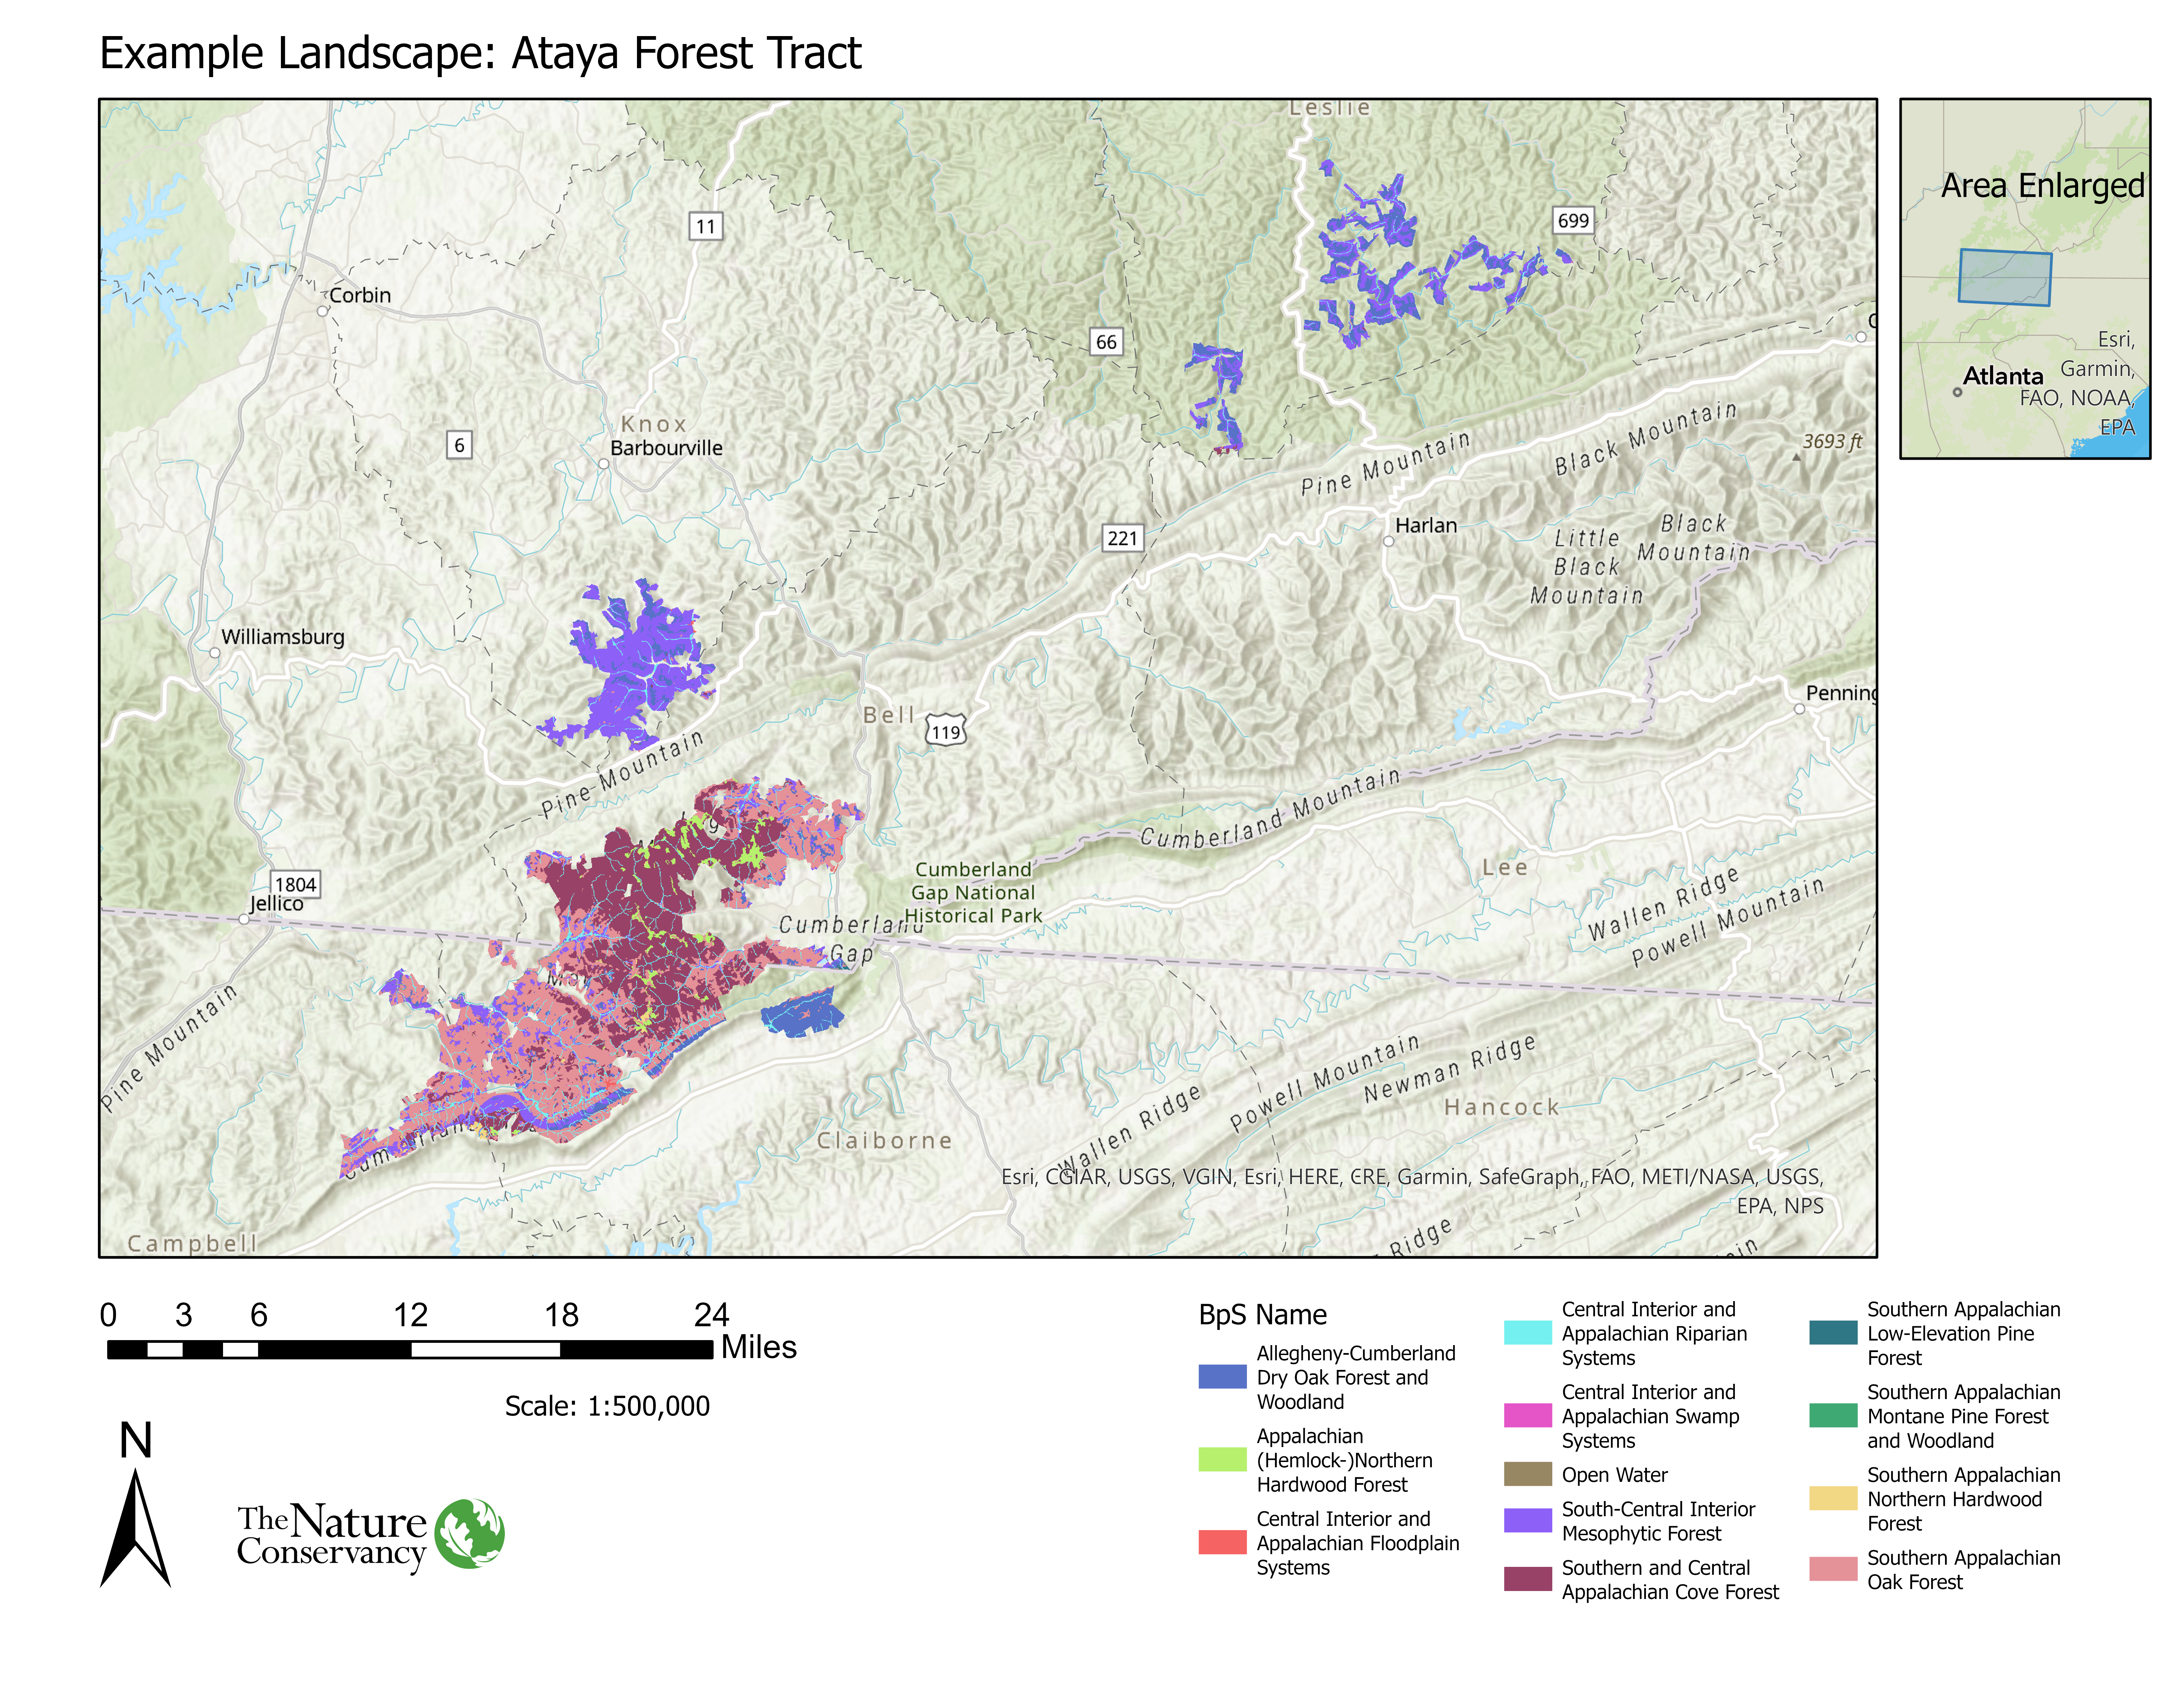
\includegraphics[width=2500px]{KP_GISmaps/Ataya_studyfig}

\hypertarget{ourmethods}{%
\chapter{Our Method}\label{ourmethods}}

\hypertarget{gis-analysis-requirements}{%
\section{GIS Analysis Requirements}\label{gis-analysis-requirements}}

This tutorial uses ESRI ArcGIS Pro (2.9). If using ArcGIS Pro, ensure your Spatial Analyst Extension is enabled. If you are unsure if this is enabled, you can check by going to Settings, Licensing, and ESRI Extensions. Once in the ESRI Extensions box, scroll down to Spatial Analyst. You will see if the license is active or ``grayed out'' (indicating you need to activate the Spatial Analyst License).

Additionally, you will need Microsoft Excel (2022) and a reliable internet connection to download the LANDFIRE datasets pertinent to this analysis.

Lastly, prior to beginning this analysis, we recommend that you create a new ArcGIS Pro project with a project specific geodatabase (named to your choosing!) If you are following the Ataya Study Area tutorial, please save that Study Area shapefile to your geodatabase. You'll be able to acquire an Ataya shapefile at the end of this section. Alternatively, if you are using your own Study Area shapefile, save it to your project specific geodatabase as you follow along with this tutorial.

\hypertarget{methods}{%
\section{Methods}\label{methods}}

Each subsequent chapter outlines steps to complete a different component of the GIS analysis. The general components of the analysis are:

\begin{itemize}
\tightlist
\item
  Downloading and preparing the necessary LANDFIRE datasets for a Study Area.
\item
  Spatially combining these LANDFIRE datasets into one (1) new Study Area LANDFIRE dataset.
\item
  Performing ``Join Fields'' to update the new Study Area Landfire dataset.
\item
  Assessing acreage of the Study Area LANDFIRE dataset and ``masking'' it to the Study Area boundary.
\item
  Performing data summary Excel steps to observe acreage of: historic ecosystems, current vegetation types, ecosystem conversion, and succession classes within the Study Area.
\end{itemize}

\hypertarget{disclaimers}{%
\section{Disclaimers}\label{disclaimers}}

There are always many different ways to complete a GIS analysis and because of this, we'd like to share a few disclaimers.

First, this tutorial is specific to the Ataya Study Area and outlines steps exactly performed to this Study Area. If you are using a different Study Area, you will have to locate the relevant LANDFIRE datasets and Biophysical Settings (BpS) descriptions for your Study Area through the LANDFIRE website.

Second, LANDFIRE data is best represented at coarse landscape scales (i.e.~landscapes in excess of 100,000 acres or more). LANDFIRE data is not as accurate for fine landscape level assessments (i.e.~a forest stand of 100 acres or less). Due to the development of LANDFIRE data at large landscape scales, some LANDFIRE ecosystem data, such as Existing Vegetation Type (EVT), may not represent a 1:1 relation of the GIS data to current ground conditions. We like to think of our analysis as a guide for understanding forest conditions past and present. This guide still functions best with human input on the ground to make effective final forest management decisions. If you have smaller acreage of forest land and still wish to perform this analysis, consider using the watershed your forest is in!

Third, this tutorial GIS analysis was performed using ArcGIS Pro only. Unfortunately for managers who are using older versions of ArcMap or open source GIS/data processing software (i.e.~GRASS GIS, QGIS) this tutorial is not designed for these GIS platforms. These platforms can likely recreate the outcomes of this tutorial, however specific geoprocessing tools may look or act differently. If using software other than ArcGIS Pro, make sure to understand the underlying process behind each tool.

If you are having trouble with this tutorial, here are some people that can assist you!

\begin{itemize}
\tightlist
\item
  Problems with LANDFIRE data? \href{mailto:helpdesk@landfire.gov}{\nolinkurl{helpdesk@landfire.gov}}
\item
  Problems with the rMarkdown document? Randy Swaty: \href{mailto:rswaty@tnc.org}{\nolinkurl{rswaty@tnc.org}}
\item
  Problems with the GIS analysis? Keith Phelps: \href{mailto:kpphelp@clemson.edu}{\nolinkurl{kpphelp@clemson.edu}} or Stacey Marion: \href{mailto:stacmarion@gmail.com}{\nolinkurl{stacmarion@gmail.com}}
\end{itemize}

We are always looking for ways to improve our GIS analysis steps, accessibility of our content, and availability of this analysis to as many forest managers as possible. If you have any suggestions for us, please reach out to Keith Phelps (\href{mailto:kpphelp@clemson.edu}{\nolinkurl{kpphelp@clemson.edu}}), Stacey Marion (\href{mailto:stacmarion@gmail.com}{\nolinkurl{stacmarion@gmail.com}}), or Randy Swaty (\href{mailto:rswaty@tnc.org}{\nolinkurl{rswaty@tnc.org}}).

\hypertarget{lastly-download-this}{%
\section{Lastly\ldots{} Download this!}\label{lastly-download-this}}

To work through this guide you will need to download this \href{https://github.com/rswaty/landfireFSC/blob/main/toDownload.zip}{zipped folder} by clicking the hyperlinked text, then the ``Download'' button that will be on the right side of the screen. This folder contains:

\begin{itemize}
\tightlist
\item
  An Ataya shapefile
\item
  An Excel file
\item
  One ecosystem description
\item
  An ArcPro map package file in case you want to explore in ArcPro.
\end{itemize}

\hypertarget{about-this-document}{%
\section{About this document}\label{about-this-document}}

It was written in R using \href{https://rstudio.com/}{R-Studio}, the \href{https://www.bookdown.org/}{``bookdown'' package} and is hosted on \href{https://github.com/rswaty/landfireFSC}{GitHub(links to this repository)}.

\hypertarget{inputdata}{%
\chapter{LANDFIRE Data for FSC®}\label{inputdata}}

\hypertarget{landfire-for-landscape-ecosystem-assessment}{%
\section{LANDFIRE for Landscape Ecosystem Assessment}\label{landfire-for-landscape-ecosystem-assessment}}

To support assessment of a forest's conditions, particularly FSC® Principles 6 - Environmental Impact \& 9 - Maintenance of High Conservation Value Forests, we consider:

\begin{itemize}
\tightlist
\item
  Change between historical and current ecosystem condition
\item
  The representation of ecosystems within and outside of your landscape of interest.
\item
  Change in Succession Classes (aka seral states) of communities over time
\end{itemize}

These steps, while foundational and conceptually simple, can be difficult due to a lack of data, especially when the study area of interest is large scale, occurs across multiple land ownerships, or is subject to land cover change. Using LANDFIRE spatial models overcomes this data barrier by providing a suite of terrestrial data appropriate for landscape scale analysis.

\hypertarget{landfire-datasets-used-for-this-tutorial}{%
\section{LANDFIRE Datasets Used For This Tutorial}\label{landfire-datasets-used-for-this-tutorial}}

\begin{itemize}
\tightlist
\item
  Spatial datasets, clipped to your area(s) of interest

  \begin{itemize}
  \tightlist
  \item
    \href{https://www.landfire.gov/bps.php}{Biophysical Settings (BpS)}. This dataset will be used to look at ``community habitat'', or where ecosystems could occur based on abiotic factors (e.g., soils, climate and natural disturbance regimes).
  \item
    \href{https://www.landfire.gov/sclass.php}{Succession classes}. This dataset characterizes structural classes on the landscape at the time the dataset represents (e.g., 2016 for LF Version 200).
  \item
    \href{https://www.landfire.gov/evt.php}{Existing Vegetation Type}. This dataset maps NatureServe's Ecological Systems (see descriptions \href{https://www.landfire.gov/documents/LANDFIRE_Ecological_Systems_Descriptions_CONUS.pdf}{here}).
  \end{itemize}
\item
  Non-spatial products

  \begin{itemize}
  \tightlist
  \item
    \href{http://landfirereview.org/test/search.php}{Biophysical Settings Descriptions} These descriptions have information on natural disturbance regimes and succession class descriptions (also available \href{https://www.landfire.gov/zip/LANDFIRE_CONUS_SClass_Mapping_Rules_9182020.zip}{here}).\\
  \item
    \href{https://www.landfire.gov/zip/LANDFIRE_CONUS_Reference_Condition_Table_August_2020.zip}{Reference Condition Table} supplements the BpS descriptions with the ``reference'' percentages for each succession class, for each Biophysical Settings.
  \end{itemize}
\end{itemize}

\hypertarget{guidance-on-obtaining-landfire-products}{%
\section{Guidance on Obtaining LANDFIRE Products}\label{guidance-on-obtaining-landfire-products}}

There are multiple ways to get LANDFIRE products depending on whether you are looking to obtain BpS models, their descriptions, or the spatial data:

\begin{itemize}
\tightlist
\item
  For BpS models and descriptions go to: \url{http://landfirereview.org/search.php}. Start by clicking on the ``View map of LANDFIRE Map Zones''. This will help you narrow down your search. Alternatively, you can wait to download BpS descriptions until you do some GIS work and get specific names of BpSs of interest.
\item
  For the spatial datasets you can explore options \href{https://www.landfire.gov/getdata.php}{here} which include:

  \begin{itemize}
  \tightlist
  \item
    Downloading \href{https://www.landfire.gov/version_comparison.php}{Full Extent Mosaics}. When you do use this option you get large files that cover the entire lower 48, AK or HI (depending on your selection). We use this method when we have several landscapes and/or a large area and no computer storage issues.
  \item
    Using the \href{https://www.landfire.gov/viewer/}{LANDFIRE Data Distribution Site}. With this method you essentially select the datasets you need then draw a rectangle (or you can select state or counties) around your area of interest to start the downloader. We recommend this if your area of interest is not too large and/or you have a low number of landscapes and/or have storage limits.
  \end{itemize}
\end{itemize}

\textbf{If you still need more assistance in downloading LANDFIRE products, please see the appendix for some tips and screenshots!}

\hypertarget{gis}{%
\chapter{LANDFIRE Data for Landscape Assessment}\label{gis}}

\hypertarget{if-you-havent-already-download-this}{%
\section{If you haven't already\ldots{} Download this!}\label{if-you-havent-already-download-this}}

Download this {[}zipped folder{]} (\url{https://github.com/rswaty/landfireFSC/blob/main/toDownload.zip}) by clicking the hyperlinked text, then the ``Download'' button that will be on the right side of the screen. This folder contains:

\begin{itemize}
\tightlist
\item
  An Ataya shapefile
\item
  Folders containing the BpS, EVT, and Sclass rasters
\item
  An Excel file
\item
  One ecosystem description
\item
  An ArcGIS Pro map package file in case you want to explore in ArcPro. This map package includes the following:

  \begin{itemize}
  \tightlist
  \item
    Our Ataya shapefile
  \item
    BpS, EVT, and SClass maps for Ataya
  \item
    A combined raster file of BpS, EVT, and Sclass datasets.
  \end{itemize}
\end{itemize}

\hypertarget{load-spatial-data}{%
\section{Load Spatial Data}\label{load-spatial-data}}

Open ArcGIS Pro and create a new project using a blank map template. Move the downloaded Ataya shapefile tutorial data into your project folder.

\includegraphics[width=1000px]{04_gis_screenshots/1_load_data}

Note that Pro creates a default geodatabase with the same name as your project. We recommend saving the Ataya shapefile to your geodatabase and hereafter, save intermediate layers to your geodatabase.

\textbf{Consider your study area:} Is it appropriate to end your analysis at the shapefile boundary? If you would like information to extend beyond the study boundary, consider creating a buffer. For our tutorial, we will limit our analysis to within the provided Ataya forest tract boundary.

\hypertarget{download-three-3-landfire-rasters-for-the-study-area-bps-evt-and-sclass}{%
\section{Download Three (3) LANDFIRE Rasters for the Study Area: BpS, EVT, and sClass}\label{download-three-3-landfire-rasters-for-the-study-area-bps-evt-and-sclass}}

There are multiple ways to get LANDFIRE products.

\begin{itemize}
\tightlist
\item
  For the spatial datasets you can explore options \href{https://www.landfire.gov/getdata.php}{here}, including:
\item
  Use the \href{https://www.landfire.gov/viewer/}{LANDFIRE Data Distribution Site}. With this method you essentially select the datasets you need then draw a rectangle (or you can select state or counties) around your area of interest to start the downloader. We recommend this if your area of interest is not too large and/or you have a low number of landscapes and/or have storage limits. \emph{Recommended for this tutorial.}
\item
  Download \href{https://www.landfire.gov/version_comparison.php}{Full Extent Mosaics} to obtain large files that cover the entire lower 48, AK or HI (depending on your selection). We use this method when we have several landscapes and/or a large area and no computer storage issues.
\end{itemize}

For some LANDFIRE data products, like the BpS model, the model (spatial data) and descriptions are downloaded separately:
* For BpS models and descriptions go to: \url{http://landfirereview.org/search.php}. Start by clicking on the ``View map of LANDFIRE Map Zones''. This will help you narrow down your search. We recommend downloading descriptions for BpS models relevant to your study area.

\includegraphics[width=1000px]{04_gis_screenshots/2_view_mapzone}

Note that for this tutorial, we downloaded rasters by using the rectangle drawing tool and \emph{drew a rectangle that was larger than our Study Area}. This ensures no raster cell data is lost in our calculations. This tutorial allows us to ``cut'' out that extra area in the end. If you are downloading your own data, always make sure to draw a downloading box that is larger than your Study Area to prevent GIS errors.

Once downloaded, move the LANDFIRE data product downloads into your Pro project folder. You should have a BpS, EVT, and SCLASS folder. Each folder contains metadata, a corresponding database table, and a raster.

\includegraphics[width=500px]{04_gis_screenshots/3_fsc_pro_poject_catalog}

\hypertarget{project-to-the-appropriate-coordinate-system}{%
\section{Project to the Appropriate Coordinate System}\label{project-to-the-appropriate-coordinate-system}}

The spatial reference of the Ataya tract shapefile is NAD83\_StatePlane\_VA\_South\_FIPS\_4502\_Feet Projected Coordinate System (Geographic Coordinate System NAD 1983).

\includegraphics[width=1000px]{04_gis_screenshots/4_crs_ataya}

\begin{enumerate}
\def\labelenumi{\arabic{enumi}.}
\item
  LANDFIRE data (BpS, EVT, sClass rasters) was downloaded as ``Best Fit UTM (NAD83 Datum)'' so the Projected Coordinate System of the LANDFIRE rasters is NAD83\_UTM\_Zone\_17N (Geographic Coordinate System was GCS\_North American\_1983).
  Given the size and location of our study area, we'll use the Virginia State Plane (South) as our map coordinate system. \emph{Note: unit is feet.}
\item
  Use the Project Raster tool to project each raster to the Virginia State Plane (South) coordinate system. Save the projected raster to the project geodatabase. \emph{Since the datum is the same for State Plane and UTM, no ``Geographic Transformation'' was needed. Resampling technique was ``Nearest Neighbor'' which is preferred for categorical/discrete data. Output cell size was in feet (98.425ft. = 30m.)}
\end{enumerate}

\includegraphics[width=1000px]{04_gis_screenshots/5_raster_project}

\begin{enumerate}
\def\labelenumi{\arabic{enumi}.}
\setcounter{enumi}{2}
\tightlist
\item
  Project the BpS, EVT, and sClass Rasters \emph{(sClass projection shown above).}
\item
  These (3) new rasters can now be used to create GIS maps for:
\end{enumerate}

\begin{itemize}
\tightlist
\item
  Historical ecosystems (Bps)
\item
  Existing ecosystem types and land cover (EVT)
\item
  Succesion class maps (sClass)
\end{itemize}

\hypertarget{landfire-data-stacking}{%
\section{LANDFIRE Data Stacking}\label{landfire-data-stacking}}

The three used LANDFIRE data products (BpS, EVT, sClass) provide unique aspects of land cover information. Because each raster maintains the same 30 x 30 meter cell, we can stack the LANDFIRE rasters to gain information about each arbitrary pixel within our study area.

Before we combine the rasters, take a look at the attribute table for each raster. Details on attributes can be found at landfire.gov
Open the Combine tool. This tool can be found by running a search in geoprocessing or you can find it in the Spatial Analyst Toolbox. Run the combine tool using the (3) project LANDFIRE rasters: us\_200bps\_proj, us\_200evt\_proj, is\_200sclass\_proj. Output raster was labeled combine\_landfire and saved within the project geodatabase.

\includegraphics[width=1000px]{04_gis_screenshots/6_combine_rasters}

Open the attribute table of the combine\_landfire raster. You will notice that only the ``Value'' field was retained in the combine. Next we will perform joins to append tabular data to the combine\_landfire raster.

\includegraphics[width=1000px]{04_gis_screenshots/7_combine_noattributes}

\hypertarget{join-bps-tabular-data}{%
\section{Join BpS Tabular Data}\label{join-bps-tabular-data}}

Use the Join Field tool (found with a geoprocessing search) to permanently join BpS attributes to the combine\_landfire raster. Follow these parameters:

\begin{enumerate}
\def\labelenumi{\arabic{enumi}.}
\tightlist
\item
  Input Table = combine\_landfire
\item
  Input Join Field = us\_200bps\_proj
\item
  Join Table = us\_200bps\_proj.
\item
  Join Table Field = VALUE.
\item
  Transfer Fields = BPS\_CODE, BPS\_MODEL, BPS\_NAME, GROUPVEG. \emph{Note: selecting additional fields will prevent you from using the prepared excel pivot tables.}
\end{enumerate}

\includegraphics[width=1000px]{04_gis_screenshots/8_join_bps}

\hypertarget{join-evt-tabular-data}{%
\section{Join EVT Tabular Data}\label{join-evt-tabular-data}}

This second join is to import EVT attributes. Open the Join Field Tool again and follow these parameters:

\begin{enumerate}
\def\labelenumi{\arabic{enumi}.}
\tightlist
\item
  Input Table = combine\_landfire
\item
  Input Join Field = us\_200evt\_proj
\item
  Join Table = us\_200evt\_proj
\item
  Join Table Field = VALUE
\item
  Transfer Fields = EVT\_NAME, EVT\_PHYS. \emph{Note: selecting additional fields will prevent you from using the prepared excel pivot tables.}
\end{enumerate}

\includegraphics[width=1000px]{04_gis_screenshots/9_join_evt}

\hypertarget{join-sclass-tabular-data}{%
\section{Join sClass tabular data}\label{join-sclass-tabular-data}}

The third and final join is to import the sClass attributes. Open the Join Field tool again and follow these parameters:

\begin{enumerate}
\def\labelenumi{\arabic{enumi}.}
\tightlist
\item
  Input Table = combine\_landfire
\item
  Input Join Field = us\_200sclass\_proj
\item
  Join Table = us\_200sclass\_proj
\item
  Join Table Field = VALUE
\item
  Transfer Fields = LABEL, DESCRIPTION. \emph{Note: selecting additional fields will prevent you from using the prepared excel pivot tables.}
\end{enumerate}

\includegraphics[width=1000px]{04_gis_screenshots/10_join_sclass}

\hypertarget{crop-the-combined-raster-to-the-study-area}{%
\section{Crop the combined raster to the study area}\label{crop-the-combined-raster-to-the-study-area}}

To ``cut'' the combined raster to the boundary of our shapefile, use the Extract by Mask tool. Follow these parameters:

\begin{enumerate}
\def\labelenumi{\arabic{enumi}.}
\tightlist
\item
  Input Raster = combine\_landfire
\item
  Input Raster or Feature Mask Data = Ataya feature class
\item
  Output raster = combine\_studyArea
  \emph{Reminder: if you decided to create a buffer around your study area, use the buffered study area feature class as your feature mask.}
\end{enumerate}

\includegraphics[width=1000px]{04_gis_screenshots/11_extract}

The resultant ``combine\_studyArea raster'' will only contain pixels within the Ataya study region:

\includegraphics[width=1000px]{04_gis_screenshots/12_combine_studyArea}

We choose to maintain the shape of the original raster (default setting within Extract by Mask tool), and thus the resultant extracted raster has jagged edges. Note that area calculations using the raster will differ slightly from area calculated from the vector feature.

\includegraphics[width=1000px]{04_gis_screenshots/13_jagged_edge}

\hypertarget{calculate-area-field}{%
\section{Calculate Area Field}\label{calculate-area-field}}

Next, we will calculate area using raster pixel size for ``combine\_studyArea'' raster. Follow these steps:

\begin{enumerate}
\def\labelenumi{\arabic{enumi}.}
\tightlist
\item
  Open the combine\_studyArea attribute table.
\item
  Within the attribute table, create a new field called ``Acres''. Select ``Float'' for data type to allow decimals in the calculation for acres.
\end{enumerate}

\includegraphics[width=1000px]{04_gis_screenshots/14_add_acres_field}

\includegraphics[width=1000px]{04_gis_screenshots/15_fields_view}

\begin{enumerate}
\def\labelenumi{\arabic{enumi}.}
\setcounter{enumi}{2}
\tightlist
\item
  In the ``Acres'' field, right click on the top and scroll to ``Calculate Field''.
\item
  Select ``Python 3'' as the Expression Type.
\item
  In ``Acres ='' banner, type this expression: !Count! *9687.4806249998 / 43560.
\item
  Click ``Apply'', then ``OK''.
\end{enumerate}

\includegraphics[width=1000px]{04_gis_screenshots/16_calculate_acres}

\emph{The sum of the Acres field corresponds to the total Ataya area (\textasciitilde100,653 acres).}

\includegraphics[width=1000px]{04_gis_screenshots/17_check_area_calc}

\textbf{Understanding the Field Calculation Expression}

\begin{itemize}
\tightlist
\item
  We use raster cell size to ascertain acreage. (See: \url{https://gis.stackexchange.com/questions/106883/measuring-area-of-raster-classes}) . Our general calculation to determine acreage is {[}Pixel count of xxx unique raster value{]} x {[}Area of a pixel (feet){]} x {[}1 acre/43,560 sqft{]} = xxx acres of a specific unique raster value
\item
  !Count! is the number of raster pixels classified as a unique raster value. From our attribute table, we see that we have 549 unique raster values. These unique raster values hold unique combinations of our BpS x EVT x sClass data.
\item
  Each original raster downloaded from LANDFIRE had a cell size of 30x30m. When we projected our rasters to Virginia State Plane South FIPS 4502 Feet, we changed the units of our rasters to feet; yielding cell size of 98.425 x 98.425 feet. The area of a single pixel is 98.425 x 98.425, equaling 9,687.4806. Therefore, we multiply !Count! by 9,687.4806. This yields the square footage associated with each unique raster value for our Study Area. To convert to acres, divide by 43,560 (1 acre = 43,560 sqft).
\item
  \emph{If you are using a different unit (i.e.~meters), you must adjust this calculation accordingly.}
\end{itemize}

\hypertarget{export-combine_studyarea-attribute-table-into-a-.csv-format}{%
\section{Export combine\_studyArea attribute table into a .csv format}\label{export-combine_studyarea-attribute-table-into-a-.csv-format}}

Now we'll take our GIS attribute table and make it usable in Excel. The following steps provide instructions for turning an attribute table into a .csv file. If you want to turn the attribute table into a new excel workbook, please see the appendix.

\begin{enumerate}
\def\labelenumi{\arabic{enumi}.}
\tightlist
\item
  Within the attribute table panel, navigate to the `burger' menu on the top right, and select Export Table.
\item
  Select combine\_studyArea as the Input Rows.
\item
  Next, select a folder location to export your table. Save the table as a logical name, such as ataya\_attributes with the .csv appendage. You must manually add the .csv appendage to export as a csv.
\end{enumerate}

\includegraphics[width=1000px]{04_gis_screenshots/18_export_table}

\hypertarget{open-the-tutorial-excel-workbook}{%
\section{Open the Tutorial Excel Workbook}\label{open-the-tutorial-excel-workbook}}

Next, open the Ataya \_combineClean.xlsx in the toDownload folder containing tutorial-specific files. This template excel spreadsheet already contains the exported Ataya attribute table in the first tab. The remaining tabs contain templates for using pivot tables to summarize the Ataya attributes.

If you performed the tutorial using your own study area rather than the Ataya study area, copy your csv into the Ataya\_combineClean.xslx template spreadsheet in the place of the ataya\_attribute tab. Name the spreadsheet to better represent your study area. Next, delete the OID, BpS code, Value, and DESCRIPTION columns to match what's in our workbook.

The following sections discuss analysis of historical conditions, current conditions, land use conversion and succession classes.

\hypertarget{historicalecosystems}{%
\chapter{Historical Ecosystems}\label{historicalecosystems}}

In this section we will learn which ecosystems, and how much of each, were on our landscape historically. Before we begin, let's review our BpS GIS map and draw some quick visual conclusions:

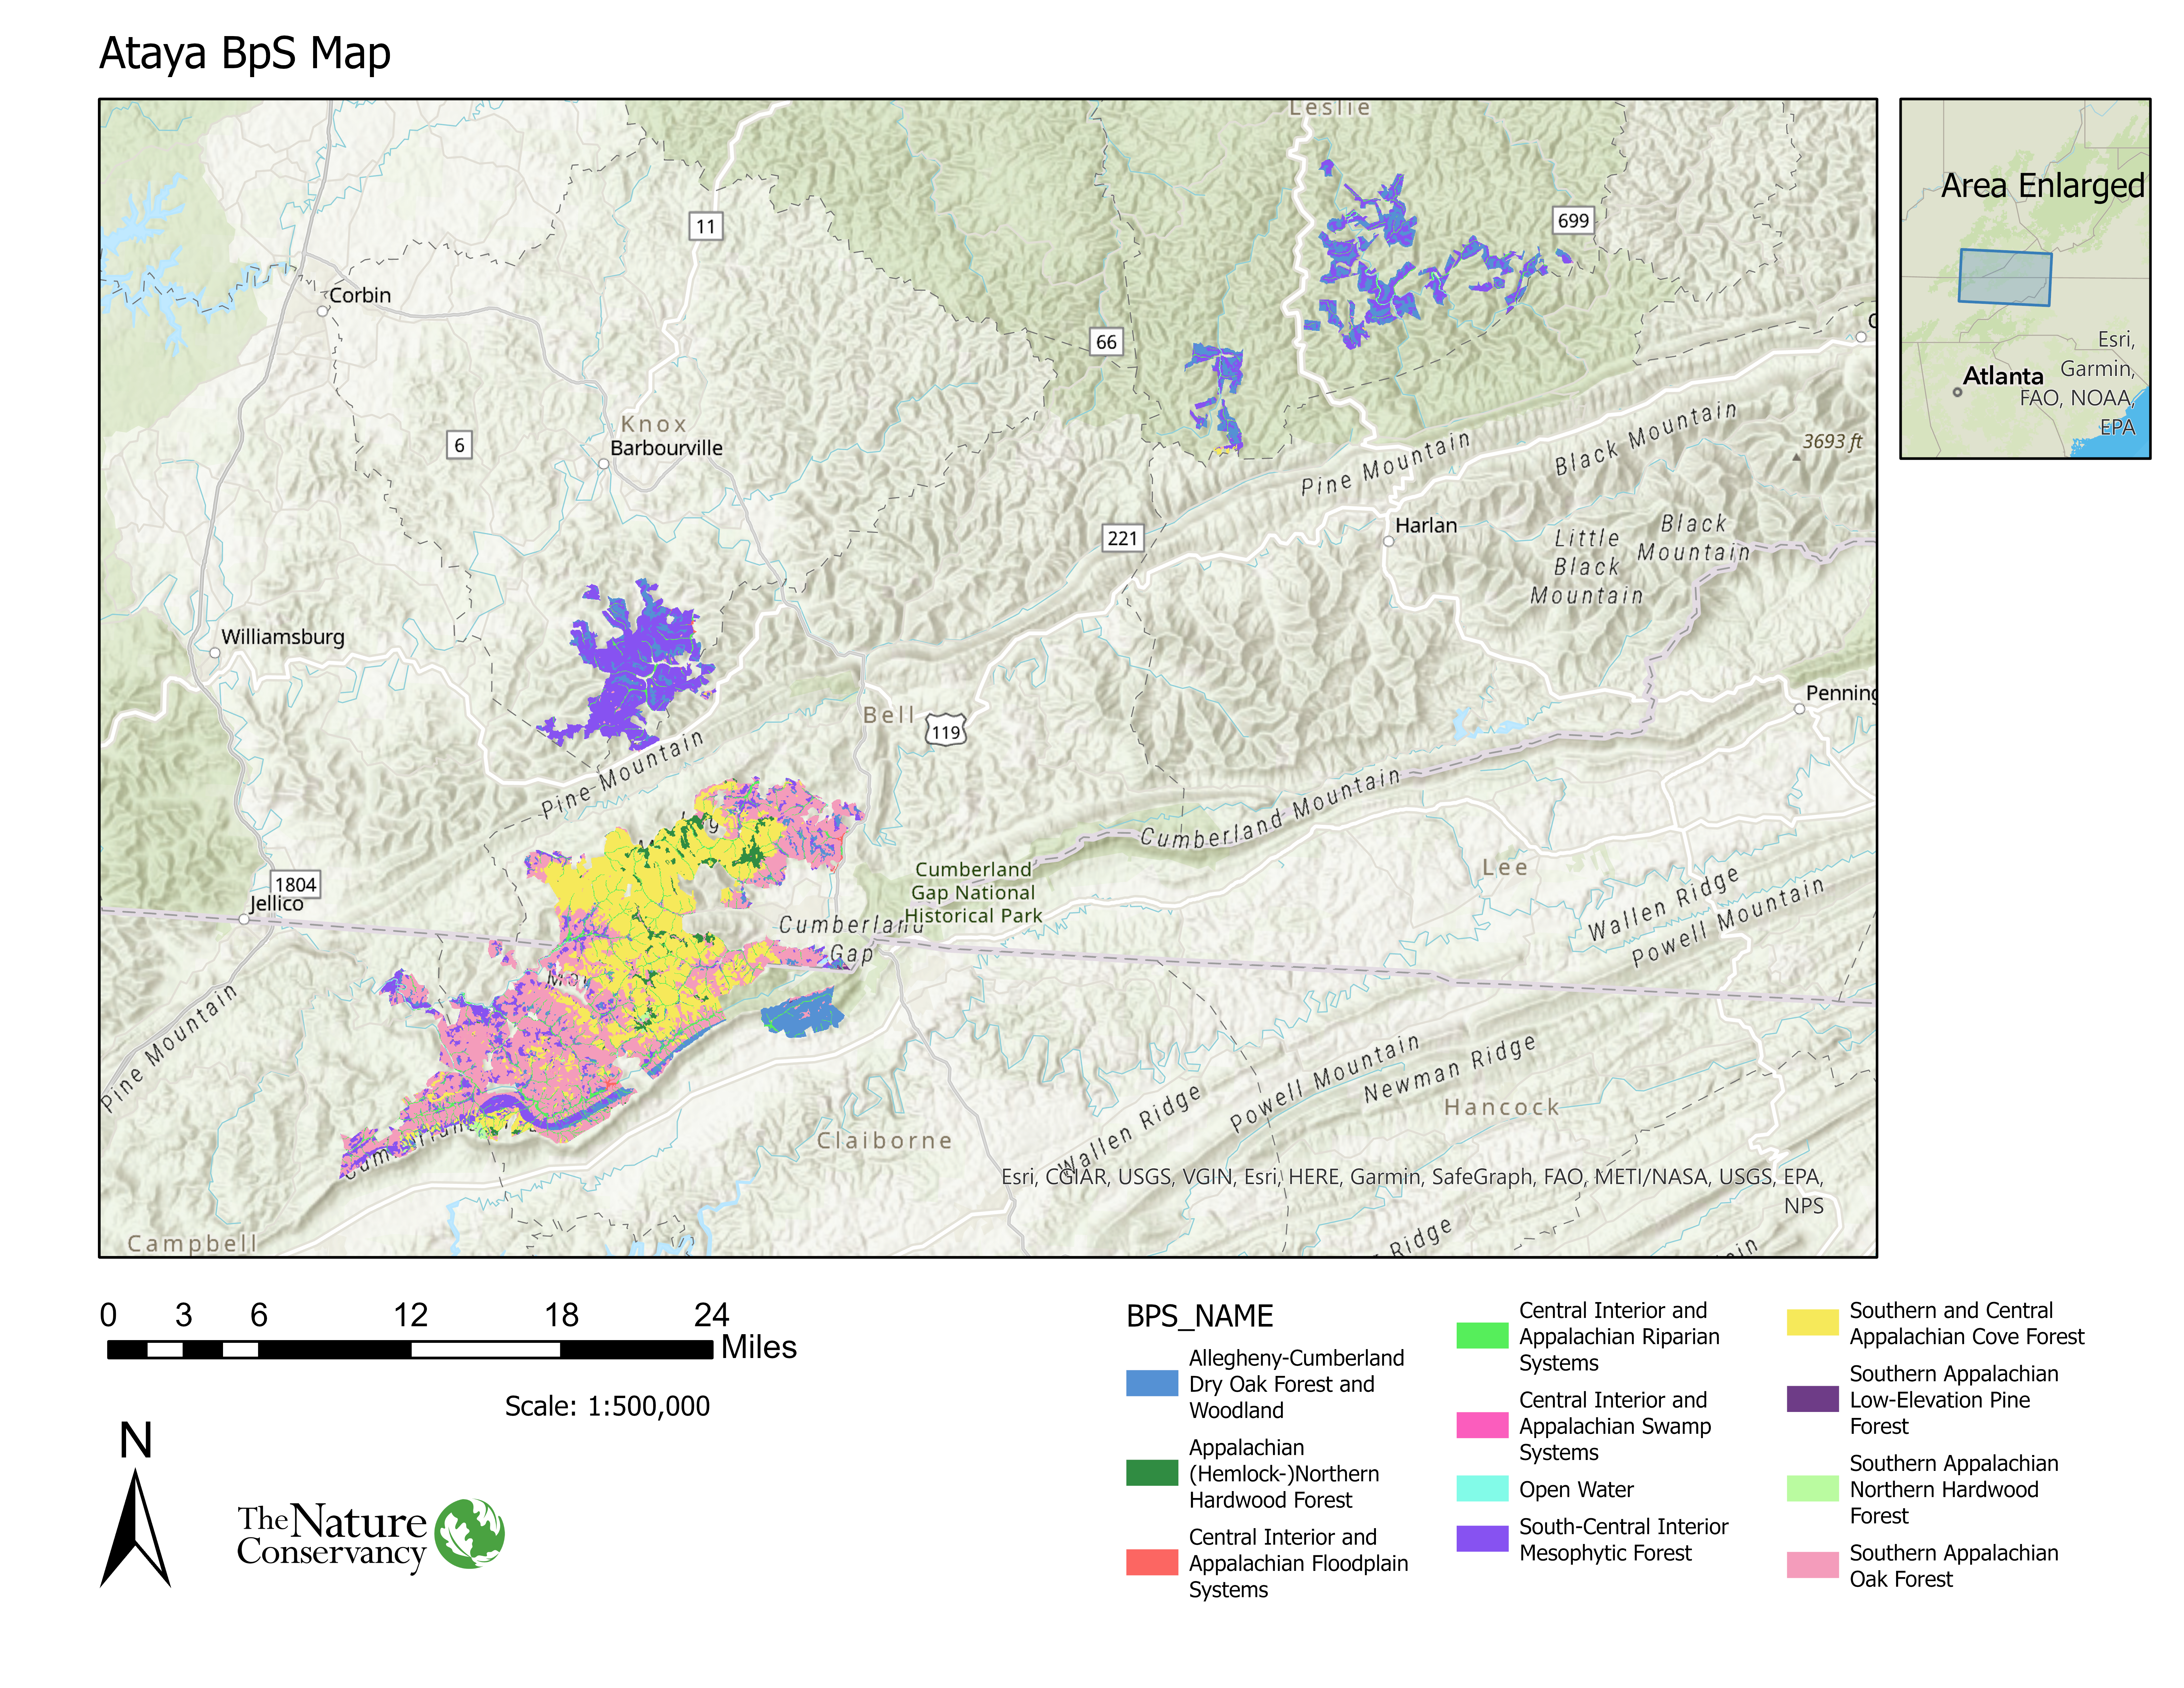
\includegraphics[width=1000px]{KP_GISmaps/Ataya_bps}

According to LANDFIRE, most of Ataya was dominated by:

\begin{itemize}
\tightlist
\item
  Southern Appalachian Oak Forest
\item
  Southern and Central Appalachian Cove Forest
\item
  South-Central Interior Mesophytioc Forest
\end{itemize}

We can also see that most of the Southern Appalachian Oak Forest and Cove Forest is confined to the southwest portions of the Study Area. In contrast, South-Central Interior Mesophytic Forests are more prevalent in the northern portions of the Study Area. Ok- let's move on!

\hypertarget{general-methods}{%
\section{General Methods}\label{general-methods}}

In this section, and most others following, we will depend on ``Pivot Tables'' in Excel. These are powerful (for better or worse!) tools that allow for tasks such as:

\begin{itemize}
\tightlist
\item
  Organization and formatting of data.
\item
  Calculations.
\item
  Filtering data.
\item
  Nesting data.
\end{itemize}

With the power comes the call for caution. It is very easy to display values that look illuminating- but may be wrong. You can easily be duped into complacency, especially when working in the ``value field settings.''

\hypertarget{some-potential-traps-with-pivot-tables}{%
\subsection{Some Potential Traps with Pivot Tables}\label{some-potential-traps-with-pivot-tables}}

Pivot Tables allow you to calculate, summarize, format and analyze datasets. These are a few traps we run into frequently which are worth mentioning here:

\begin{itemize}
\tightlist
\item
  \textbf{Your Pivot Table controls go away}. This happens when you click outside of the main Pivot Table area (where your values are, usually on the left side of screen). To fix this click inside one of the Pivot Table columns. Another way to fix this is to right click inside a Pivot Table cell and select ``Show field list''.
\item
  \textbf{Miscalculating.} This typically happens when you are in the ``Value Field Settings'' pane and select the wrong ``Show values as'' option. The key here is to visually inspect the results to make sure you have made the correct selection.
\item
  \textbf{You want to remove totals and subtotals without having to delete them all.} To fix this and many formatting issues click anywhere inside of the Pivot Table -\textgreater{} Click ``Design'' from the top ribbon -\textgreater{} click the ``Subtotals'' drop down -\textgreater{} click ``Do Not Show Subtotals''. Repeat for Grand Totals. While you are there, explore the Report Layout and Blank Rows drop downs.
\end{itemize}

\hypertarget{getting-at-amounts-of-historical-ecosystems}{%
\section{Getting at amounts of historical ecosystems}\label{getting-at-amounts-of-historical-ecosystems}}

\textbf{Start by opening the ``Historical'' tab in the Excel workbook (``combineClean'').}

\begin{enumerate}
\def\labelenumi{\arabic{enumi}.}
\tightlist
\item
  In the Pivot Table Fields pane, select ``BPS\_NAME'' then ``ACRES''.\\
\item
  Right click in the top cell of the ``Sum of ACRES'' column (not the column header) in the Pivot Table, then ``Sort Largest to Smallest''.
\item
  In our example we have some BpSs that have low ACRES values. We can do a little formatting/cleaning before making a chart:

  \begin{itemize}
  \tightlist
  \item
    To remove BpSs from the table you will click the drop-down menu to the right of ``BPS\_NAME'' in the Pivot Table Fields pane. You can uncheck BpSs as appropriate.
  \item
    It is also possible to filter by right clicking on the top value in the list of BpSs, then selecting Filter \textgreater{} Top 10\ldots. Once in that menu you can refine the filtering.
  \end{itemize}
\item
  To get percentages, drag ``ACRES'' from the top Pivot Table Field pane to the ``Values'' pane. This will add a second ``ACRES'' column to the table. Right click in the second instance of ``ACRES'' (reads ``SUM of ACRES2'' in our example) to open up a drop down menu, then navigate to Value Field Settings. In this menu select the ``Show Values As'' tab, click the ``Show Values As'' drop down then select ``\% of Grand Total\% to get percentages of each BpS (make sure that''BPS\_NAME'' is selected as the ``Base field'').\\
\item
  To get a ``running total'' of percentages you will add a third instance of ``ACRES'' to the ``Values'' pane, then navigate to Value Field Settings. In this menu select the ``Show Values As'' tab, click the ``Show Values As'' drop down then select ``\% Running Total In'' to get running totals of percentages of each BpS (make sure that ``BPS\_NAME'' is selected as the ``Base field'').
\item
  Save!
\end{enumerate}

\textbf{Example output}

Below is essentially the output from our Pivot Table work with a couple changes:

\begin{itemize}
\tightlist
\item
  Names have been shortened for ease of reading.
\item
  Numbers have been rounded.
\end{itemize}

We see that the top 3 BpSs comprised \textasciitilde80\% of our example landscape historically. We can visually confirm this and other patterns with a quick chart made in R (similar charts available in Excel by highlighting the data, clicking Insert then selecting the chart type in the ``Charts'' tab):

\includegraphics{FSCBook_files/figure-latex/bpsChart-1.pdf}

\hypertarget{evt}{%
\chapter{Existing Vegetation Types}\label{evt}}

While looking at the historical ecosystems gives context, we also need to get a picture of which ecosystems are on the landscape today. Like the last section, let's first take a look at our EVT GIS Map to draw some conclusions:

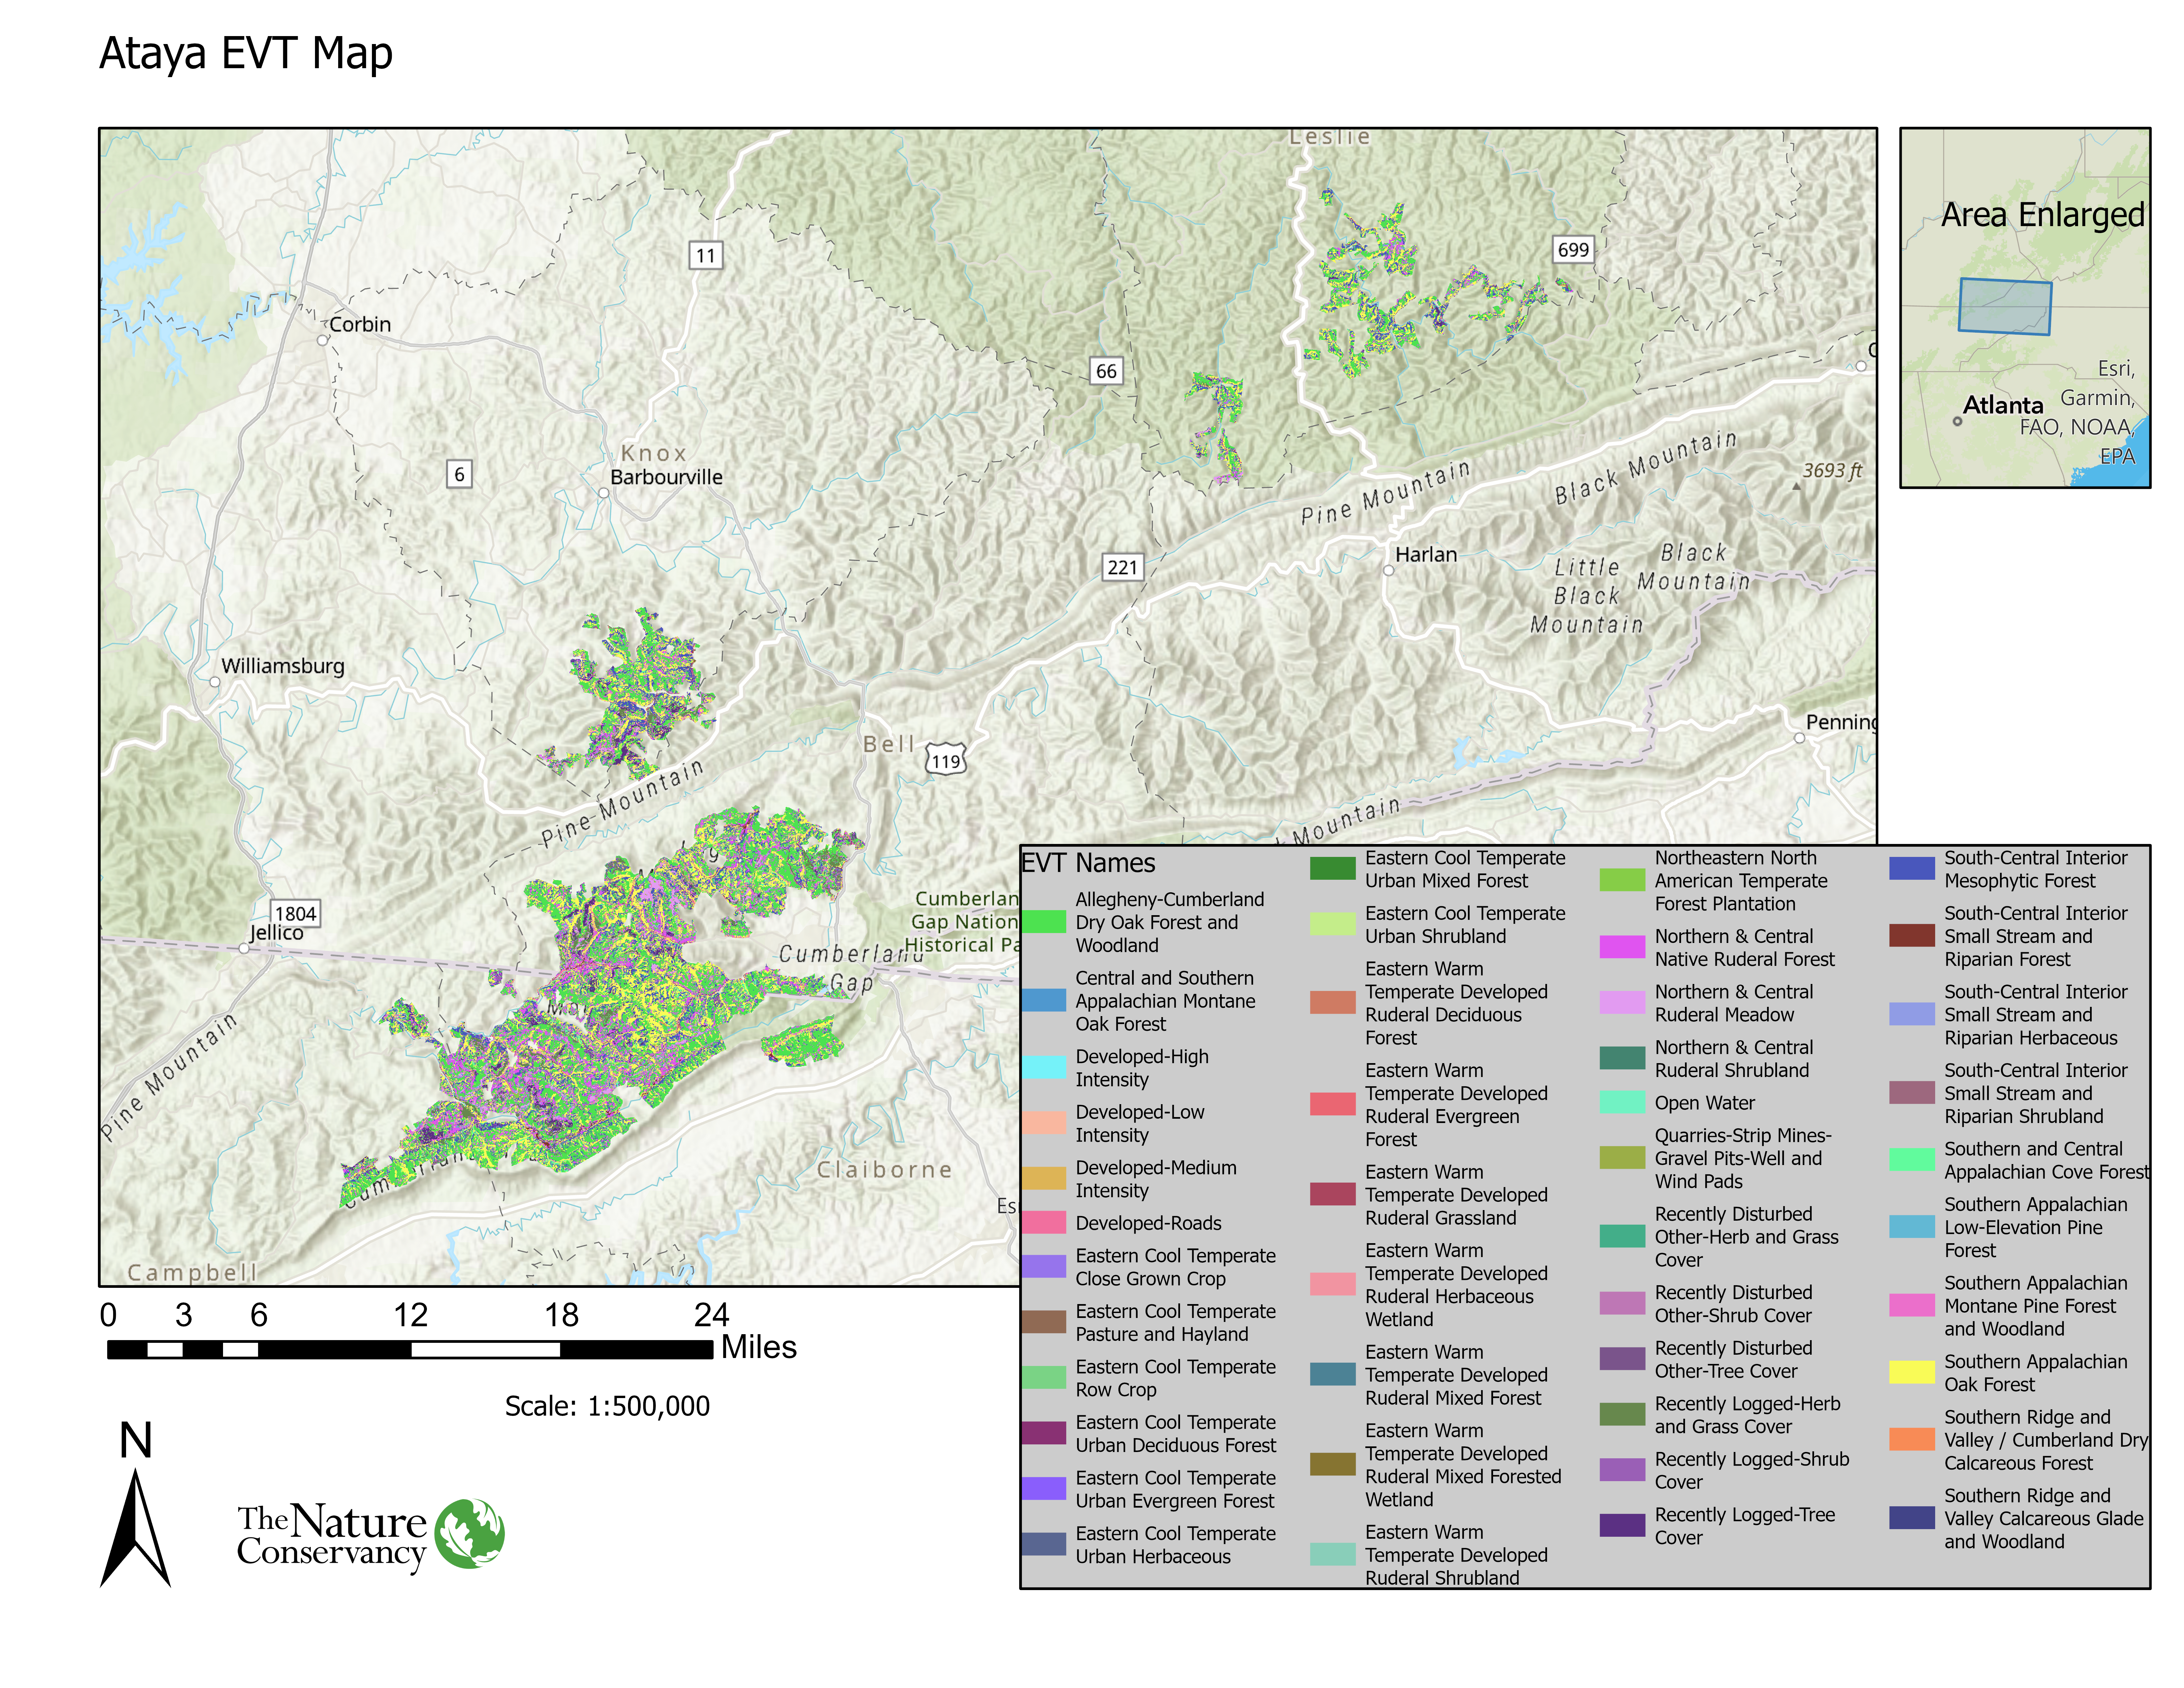
\includegraphics[width=1000px]{KP_GISmaps/Ataya_evt}

As we can see, there are FAR more ecosystem types present in Ataya today. In the map we see that there is far more Allegheny Dry Oak Forest/Woodland, Northern and Central Native Ruderal Forest, and recently logged cover. This map is certainty different from our Bps map! Let's move on\ldots{}

\hypertarget{general-methods-1}{%
\section{General Methods}\label{general-methods-1}}

We use the same general methods as we did on the ``Historical Ecosystems'' page, as we will be using another Pivot Table. We rely on \href{https://www.landfire.gov/evt.php}{LANDFIRE's Existing Vegetation Type (EVT)} data for this assessment.

\hypertarget{getting-at-amounts-of-current-ecosystems}{%
\section{Getting at Amounts of Current Ecosystems}\label{getting-at-amounts-of-current-ecosystems}}

\textbf{Start by opening the ``current'' tab in the Excel workbook.}

\begin{enumerate}
\def\labelenumi{\arabic{enumi}.}
\tightlist
\item
  In the Pivot Table Fields pane, select ``EVT\_NAME'' then ``ACRES''. Make sure that EVT\_NAME is in the ``Rows'' pane, and that ``Sum of ACRES'' is in the ``Values'' pane.\\
\item
  Right click in the top cell of the ``Sum of ACRES'' column (not the column header) in the Pivot Table, then ``Sort Largest to Smallest''.
\item
  In our example we have some BpSs that have low ACRES values. We can do a little formatting/cleaning before making a chart:

  \begin{itemize}
  \tightlist
  \item
    To remove EVTs from the table you will click the drop-down menu to the right of ``BPS\_NAME'' in the Pivot Table Fields pane. You can uncheck BpSs as appropriate.
  \item
    It is also possible to filter by right clicking on the top value in the list of EVTs within the Pivot Table, then selecting Filter \textgreater{} Top 10\ldots. Once in that menu you can refine the filtering.
  \item
    Additionally, we would like to add commas and remove decimal places. To do this right click the row that contains ``Sum of ACRES'' in the spreadsheet (likely row ``B''), select ``Format Cells'' \textgreater{} Number \textgreater{} set Decimal places to ``0'' then check the ``Use 1000 Separator box.
  \end{itemize}
\item
  To get percentages, drag ``ACRES'' from the top Pivot Table Field pane to the ``Values'' pane. This will add a second ``ACRES'' column to the table. Right click to open up the drop down in the second instance of ``ACRES'' (reads ``SUM of ACRES2'' in our example), then navigate to Value Field Settings. In this menu select the ``Show Values As'' tab, click the ``Show Values As'' drop down then select ``\% of Grand Total\% to get percentages of each EVT (make sure that''EVT\_NAME'' is selected as the ``Base field'').\\
\item
  To get a ``running total'' of percentages you will add a third instance of ``ACRES'' to the ``Values'' pane, then Value Field Settings. In this menu select the ``Show Values As'' tab, click the ``Show Values As'' drop down then select ``\% Running Total In'' to get running totals of percentages of each BpS (make sure that ``BPS\_NAME'' is selected as the ``Base field'').
\item
  Save!
\end{enumerate}

\textbf{Example output}

Below is essentially the output from our Pivot Table work with a couple changes:

\begin{itemize}
\tightlist
\item
  Names have been shortened for ease of reading
\item
  Numbers have been rounded
\item
  We have only included a selection of (5) EVTs
\end{itemize}

We see that first there are many EVT's. This is partially due to the addition of Developed and other ``modern'' categories such as ``Recently Logged-Tree Cover''. Second we see that of the ``natural'' types there are some important changes from historic ecosystem conditions. In Ataya, there is currently far more acreage associated with Allegheny Dry Oak Forest/Woodland. We can visually confirm this and other patterns with a quick chart made in R (similar charts available in Excel by highlighting the data, clicking Insert then selecting the chart type in the ``Charts'' tab):

\includegraphics{FSCBook_files/figure-latex/evtChart-1.pdf}

\hypertarget{conversion}{%
\chapter{Exploring Conversion}\label{conversion}}

\textbf{The main question we explore on this page: how much of the historic ecosystems have been converted to a different land use or ecosystem type? (e.g., agriculture, forest types).}

\hypertarget{the-fine-print}{%
\section{The Fine Print}\label{the-fine-print}}

While this assessment is illustrative, it is important to note that the methods used to create the BpS and EVT datasets are substantially different, and LANDFIRE datasets are not made for assessing small areas. Please review. In the exercise we will focus on the coarsest classifications. If you need to work at the finer classification levels proceed with caution!

\hypertarget{pivot-table-work}{%
\section{Pivot Table Work}\label{pivot-table-work}}

Working in the ``Conversion'' worksheet:

\begin{enumerate}
\def\labelenumi{\arabic{enumi}.}
\tightlist
\item
  Check the ``GROUPVEG'' then the ``EVT\_PHYS'' fields to add them to the Pivot Table. Make sure that GROUPVEG is the leftmost column. If not drag that field to the top in the Rows pane.
\item
  In the cell above the ``GROUPVEG'' field header type ``past''; in the cell above the ``EVT\_PHYS'' type ``present''.
\item
  If you fancy click the dropdown in the ``GROUPVEG'' header. Here you can remove types.
\item
  Check the ``ACRES'' field to add it to the Pivot Table.
\item
  Explore. Of what was historically mapped as CONIFER, what's the biggest non-CONIFER type today?
\item
  Switch the order of the fields by dragging ``EVT\_PHYS'' to the top of the Rows pane. Which GROUPVEG type was most converted to ``Developed''?
\end{enumerate}

We can easily make excel charts and bar graphs to summarize these findings and demonstrate change from historic conditions. We can also dive a little bit deeper to generate a table that illustrates percent change from historic ecosystem conditions to current ecosystem conditions.

\hypertarget{excel-steps-for-preparing-an-ecosystem-conversion-table}{%
\section{Excel Steps for Preparing an Ecosystem Conversion Table}\label{excel-steps-for-preparing-an-ecosystem-conversion-table}}

Here are steps to create a table summary which will allow us to view percent change of historical ecosystems (Bps) into current ecosystems (EVT):

\begin{enumerate}
\def\labelenumi{\arabic{enumi}.}
\tightlist
\item
  Open the ``Bps2evt'' worksheet
\item
  In the Pivot Table, check ``BPS\_Name'', ``EVT\_Name'', and ``COUNT''
\item
  In the Main Ribbon of the worksheet (where File, Home, Insert, etc. are located) navigate all the way to the last Tab on the right labeled ``Design''. Click on ``Design''.
\item
  In the ``Subtotals'' tab, click on the down arrow and navigate to ``Do Not Show Subtotals''. Click on this option.
\item
  In the ``Grand Totals'' tab, click on the down arrow and navigate to ``Turn Off for Rows and Columns''. Click on this option.
\item
  In the ``Report Layout'' tab, click on the down arrow and navigate to ``Show In Tabular Form''. Click on this option.
\item
  In the ``Report Layout'' tab, click on the down arrow and navigate to ``Repeat All Item Labels''. Click on this option.
\item
  In the top data cell for the ``BPS\_Name'' data column, right click and navigate to ``Filter''. Click on ``Top 10\ldots{}''
\item
  In the box that opens, change ``10'' to 90 and ``Items'' to ``Percent''.

  \begin{itemize}
  \tightlist
  \item
    This will select the top 90\% of BpS settings in the Ataya Study Area. To display all BpS, we would type in 100.
  \end{itemize}
\item
  In the top data cell for the ``EVT\_Name'' data column, right click and navigate to ``Filter''. Click on ``Top 10\ldots{}''
\item
  In the box that opens, change ``10'' to 90 and ``Items'' to ``Percent''.

  \begin{itemize}
  \tightlist
  \item
    This will select the top 90\% of EVT settings in the Ataya Study Area. To display all EVTs, we would type in 100.
  \end{itemize}
\item
  In the ``Sum of Count'' data column, right click on the top cell and navigate to ``Value Field Settings''.
\item
  In ``Value Field Settings'', click on ``Show Values As'' and navigate to ``\% of Parent Row total'' and click.
\item
  Change the name of ``Sum of Count'' to ``Percent''.
\end{enumerate}

Voila! We now have a table which should look similar to what's below. For this tutorial, we have rounded our percents and are only displaying a portion of the table for better website viewing.

\hypertarget{interpreting-the-ecosystem-conversion-table}{%
\section{Interpreting the Ecosystem Conversion Table}\label{interpreting-the-ecosystem-conversion-table}}

This table gives us a general idea of the percent change from historic ecosystems into current ecosystems. In our table above, we see that 57\% of historic Allegheny-Cumberland Dry Oak Forest/Woodland has remained as this ecosystem type within Ataya. We also see that 14\% of Allegheny-Cumberland Dry Oak Forest/Woodland has converted into Northern \& Central Ruderal Forest (a forest type marked by ``weedy'' generalist species). Additionally, 29\% of South-Central Interior Mesophytic Forest has converted into Alleghany-Cumberland Dry Oak Forest/Woodland.

Here is a potential ecological interpretation for the Ecosystem Conversion Table results of our Study Area (partially based on the table and partially based on local knowledge):

\begin{itemize}
\tightlist
\item
  There is far more Allegheny Dry Oak Forest and Northern/Central Native Ruderal Forest mapped today than historically. Additionally, Southern Appalachian Cove and South-Central Interior Mesophytic Forests have greatly decreased over time. This could be due to a legacy of extensive ecosystem disturbance on the landscape. For example, we know that extensive clear-cut logging occurred all throughout the Appalachians in the late 19th and early 20th centuries. After these cut-over events, extensive wildfires erupted across the region due to the residual logging slash. These wildfires also spawned US Forest Service fire suppression policies in the early 20th century which altered ecosystem disturbances further.
\item
  One hypothesis would be that due to homogeneous logging and wildfire disturbance across large landscape contexts, favorable conditions to shade-intolerant oak species (i.e.~high light levels, open canopies, reduced duff layers) resulted in a massive increase in oak recruitment. As the forests grew back, oak became a far more common tree species and influenced the development of forest types away from maples, tulip-poplars, and other more shade-tolerant trees- typical dominants of Southern Appalachian Cover and South-Central Interior Mesophytic Forests. Additionally, as American chestnuts were lost due to chestnut blight in the early 20th century, oaks most likely took their place.
\end{itemize}

We can also dive EVEN FURTHER by visualizing these ecosystem changes\ldots{}

\hypertarget{visual-exploration-with-a-sankey-diagram}{%
\section{Visual Exploration with a Sankey Diagram}\label{visual-exploration-with-a-sankey-diagram}}

Sometimes patterns emerge more explicitly from visuals. Below is a \href{https://en.wikipedia.org/wiki/Sankey_diagram}{Sankey Diagram} generated in R (which can also be created in Excel we hear. See instructions \href{https://mychartguide.com/how-to-draw-sankey-diagram-in-excel/}{here}). We used the data from our Conversion Table above to create this R figure. On the left are the historical ecosystems, on the right current ecosystems and flow bands. The width of the bands is proportional to the flow rate.

Click \href{https://rswaty.github.io/landfireFSC/sankey.html}{here} to the view diagram in your web browser.

\hypertarget{successionClasses}{%
\chapter{Succession Classes}\label{successionClasses}}

\hypertarget{what-we-will-do}{%
\section{What We Will Do}\label{what-we-will-do}}

While looking at conversion of historical ecosystems is valuable, we can perform more analyses, comparing amounts historical succession classes to current. This gives us a broad measure of the changes in vegetation structure for ecosystems.

\hypertarget{what-are-succession-classes}{%
\section{What are ``Succession Classes?''}\label{what-are-succession-classes}}

In general LANDFIRE succession classes are stages of development defined in the descriptions of each Biophysical Setting. They are characterized by vegetation height, canopy cover and to some degree species composition. Key takeaways:

\begin{itemize}
\tightlist
\item
  To learn what the succession classes are for each Biophysical Setting you look to the corresponding description on \url{http://landfirereview.org/test/search.php}
\item
  LANDFIRE used state and transition models to estimate the amount of each succession class that would occur with natural (pre-European colonization) disturbance regimes. Historical succession classes were not mapped as they were assumed to move around over time.
\item
  The \href{https://www.landfire.gov/sclass.php}{Succession Class} dataset maps the current location of succession classes, in addition to agricultural and developed land-use classes plus uncharacteristic vegetation. Uncharacteristic typically represents exotic vegetation, or vegetation structure that would not have occurred historically.
\item
  By comparing the amounts of historical and current succession classes you can get a sense of which classes are over/under represented. This assumes that the landscape you are assessing is large enough to potentially include the full compliment of succession classes.
\end{itemize}

\hypertarget{our-sample-ecosystem}{%
\section{Our Sample Ecosystem}\label{our-sample-ecosystem}}

First, let's take another look at our sClass GIS map for some visual context:

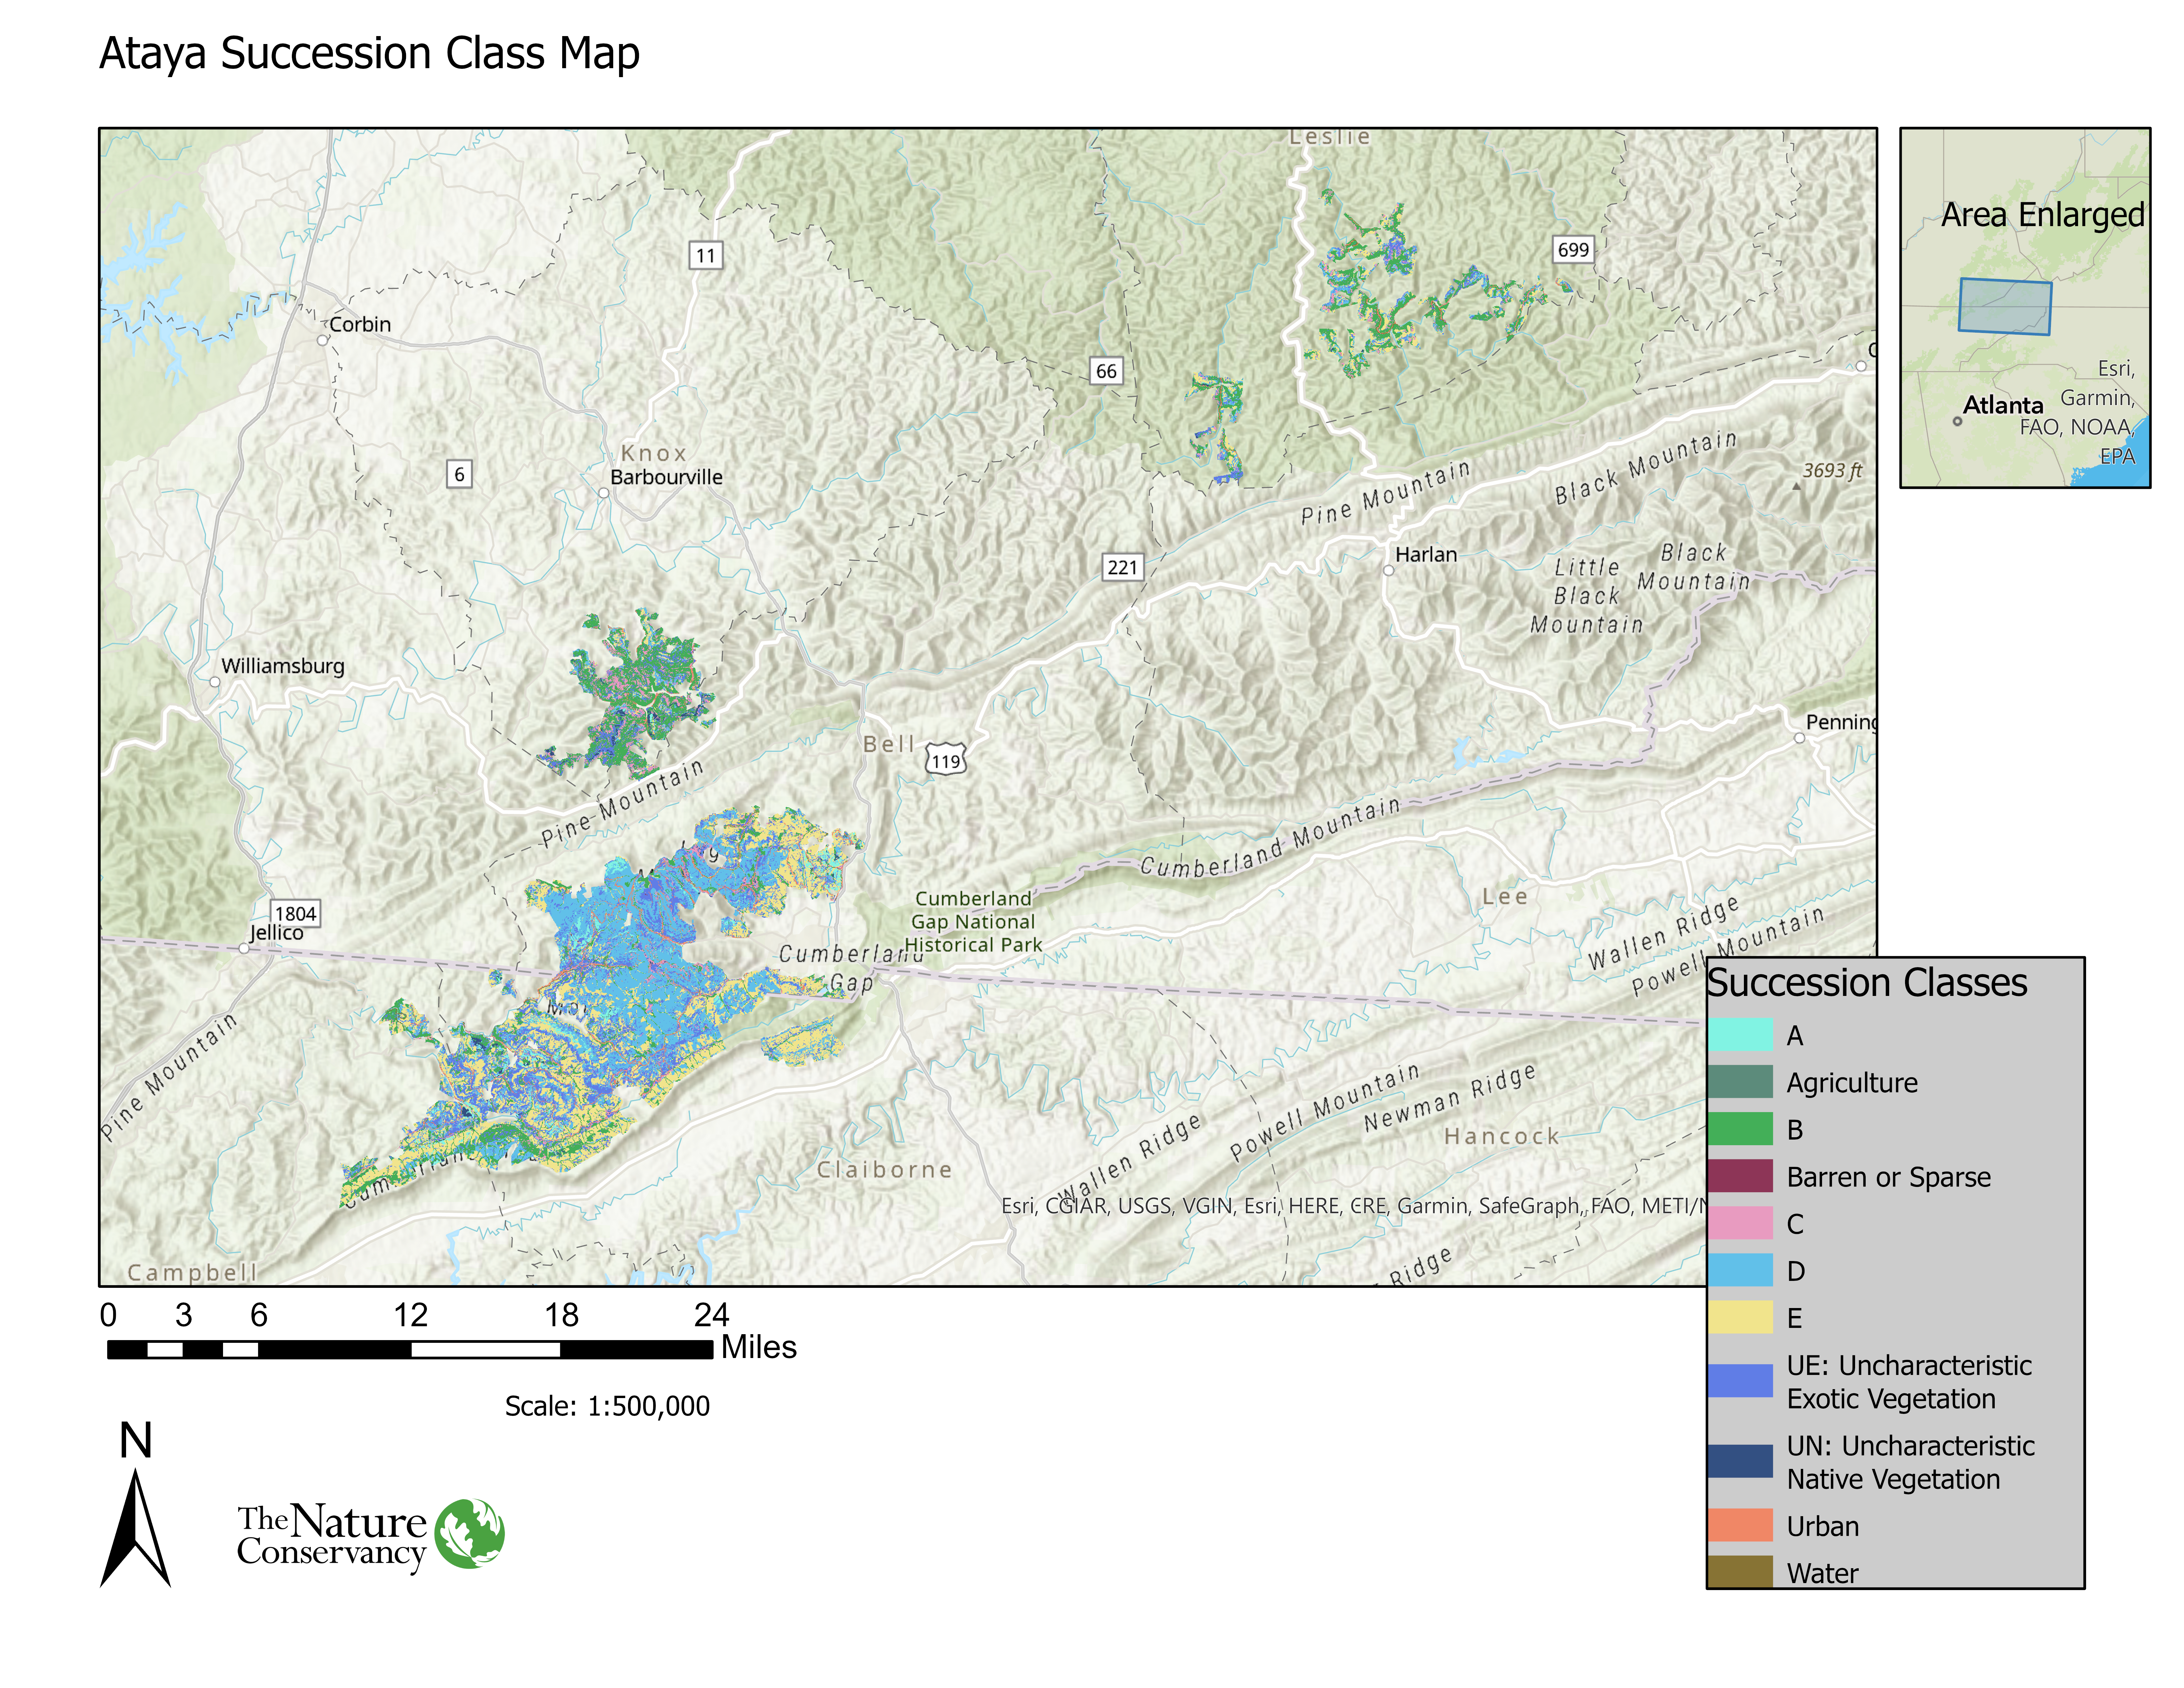
\includegraphics[width=1000px]{KP_GISmaps/Ataya_sclass}

We see that most of the succession classes in Ataya are in Succession Class B, D, and E. There is also a large amount of area devoted to UE: Uncharacteristic Exotic Vegetation.

To illustrate the concept of comparing reference to current succession classes, we will focus on the South-Central Interior Mesophytic Forest Biophysical Setting. It is a dominant ecosystem in the Ataya, has been heavily managed, has experienced extensive clear cut logging, and faces many threats such as deer browsing (and in isolated pockets hemlock woody adelgid damage).

\hypertarget{your-tasks}{%
\section{Your Tasks}\label{your-tasks}}

We will start with our friend the Pivot Table to get current percentages of the relevant succession classes, then we will look to the Biophysical Settings descriptions to get historical percentages.

\hypertarget{current-succession-classes}{%
\subsection{Current Succession Classes}\label{current-succession-classes}}

\begin{enumerate}
\def\labelenumi{\arabic{enumi}.}
\tightlist
\item
  Open the ``successionClasses'' worksheet in our ``Ataya\_combineClean.xlsx'' workbook.
\item
  In the Pivot Table Fields box highlight ``BPS\_MODEL'' -\textgreater{} click the down arrow -\textgreater{} select only ``South-Central Interior Mesophytic Forest''. Check the box next to ``BPS\_NAME''.
\item
  In the Pivot Table Fields check the box next to ``LABEL'' to get a list of current succession classes.
\item
  In the Pivot Table Fields check the box next to ``ACRES''.
\item
  In the Values pane click the down arrow -\textgreater{} select Value Field Settings. Once the Value field settings are open click Show Values As -\textgreater{} select ``\% of Grand Total'' from the dropdown list.
\item
  Copy the resultant table -\textgreater{} paste next to the Pivot Table in the same worksheet -\textgreater{} add column names ``Succession class'' and ``Current''.
\end{enumerate}

\hypertarget{historical-succession-classes}{%
\subsection{Historical succession classes}\label{historical-succession-classes}}

\begin{enumerate}
\def\labelenumi{\arabic{enumi}.}
\tightlist
\item
  Open the ``SouthMesophytic.docx'' document that is in the ``toDownload'' zipped folder.\\
\item
  Skim through the document to get a sense of the ecosystem, paying particular attention to the ``Succession Classes'' section.
\item
  There are be 5 succession classes, A, B, C, D and E with corresponding estimated reference amounts. For example, Succession Class A was modeled to be rare in this ecosystem as fire was infrequent with the average fire return interval for the ecosystem being 50-200 years. LANDFIRE estimated that only 2\% of this ecosystem would have been Succession Class A historically.
\item
  Back in the pivot table, you will create a new column named ``Historical'', then type the succession class percentages from the document into the corresponding row.
\end{enumerate}

Now we can start to see some patterns emerge. What do you see and can you draw any conclusions for forest management within the Ataya? We won't spoil your fun by saying what those patterns are!

\hypertarget{conclusions}{%
\chapter{Conclusions}\label{conclusions}}

\hypertarget{bringing-it-all-together}{%
\section{Bringing it All Together}\label{bringing-it-all-together}}

We've got a lot of useful deliverables from our analysis (GIS maps, tables, charts, interpretations) but let's spend some time bringing all our analyses together. For Ataya, we see that historically our forest was dominated mostly by Southern Appalachian Oak Forest, Southern and Central Appalachian Cove Forest, and South-Central Interior Mesophytic Forests. We also know the current forests have shifted most to Allegeheny Dry Oak Forest/Woodland. Southern and Central Appalachian Cove Forests have experienced a particularly high degree of ecosystem conversion. Additionally, Ataya has large areas of uncharacteristic exotic vegetation and native ruderal forest.

\textbf{Let's draw some potential forest management implications.}

This is not an exhaustive list by any means- just some ideas to get the creative juices flowing. Feel free to revisit our previous sections to view GIS maps and charts!

\begin{itemize}
\tightlist
\item
  We see a very high departure from historic conditions for Ataya. Our restoration efforts shouldn't be focused on re-converting everything back to our BpS map as this is not feasible. This is not to say we should avoid preserving and locating unchanged forest. We can use our BpS and EVT maps to potentially find areas where the forests have remained stable for longer periods of time, and use these areas as representatives of historic conditions for teaching purposes, genotype conservation, and seed collection/preservation among other things.\\
\item
  Perhaps we need to spend some extra time mapping Cove Forest communities in the field. If this forest type is experiencing particular heavy ecosystem conversion, it may be important we assess, preserve, and more intimately manage the best representations of that forest community type.
\item
  We have a better idea of where we may need to concentrate efforts on invasive plant management. This includes areas in the southern portions of Ataya where concentrated pockets of uncharacteristic exotic vegetation can be observed. A field assessment could confirm these suspicions and influence an Integrated Pest Management plan.
\item
  We know that oaks require specific shade-reduced conditions to regenerate and recruit into the forest canopy. Based on the level of oak community types present on the landscape now, prescribed fire and timber harvesting to facilitate oak regeneration (i.e.~thinning, shelterwood cuts) will be incredibly important for a forest management plan/strategy.

  \begin{itemize}
  \tightlist
  \item
    Since most of the oak dominated forests in the south of Ataya are in Succession Class D and E (i.e.~more closed canopy conditions), prescribed fire and harvesting activities to facilitate tree canopy gaps and oak recruitment may be very important in this section of the forest.
  \end{itemize}
\end{itemize}

\hypertarget{recap-for-fsc}{%
\section{Recap for FSC®}\label{recap-for-fsc}}

After our analysis is complete, we can see that we have provided the following for a potential FSC® Audit:

\begin{itemize}
\tightlist
\item
  Maps and acreage for historic ecosystems
\item
  Maps and acreage for current ecosystems/land cover
\item
  Mapss of current Forest Succession Classes
\item
  Tables to assess ecosystem conversion
\item
  Tables to assess acreage for historic and present conditions
\item
  Some strategies for developing management implications with LANDFIRE
\end{itemize}

We hope you have enjoyed our tutorial. We wish you all the best in your future LANDFIRE analyses and keep us updated with any unique findings for your forest area!

\hypertarget{appendix}{%
\chapter{APPENDIX}\label{appendix}}

\hypertarget{landifre-data-downloading-help}{%
\section{LANDIFRE Data Downloading Help}\label{landifre-data-downloading-help}}

\textbf{LANDFIRE Data Download Homepage}

\begin{enumerate}
\def\labelenumi{\arabic{enumi}.}
\tightlist
\item
  LANDFIRE 2016 EVT data will be the default display.
\item
  You can turn off EVT layers and find different data layers on the left hand column.
\item
  Regions and bookmarks can be found/made on the right.
\end{enumerate}

\includegraphics[width=1000px]{KP_screenshots/LANDFIRE First Load}

\textbf{LANDFIRE Identify Tool}

\begin{enumerate}
\def\labelenumi{\arabic{enumi}.}
\tightlist
\item
  Click where the red arrow is pointing.
\item
  This will allow you to ID layers you have selected. Your query will be displayed in the right hand column (under ``Feature Info'').
\item
  We see that we have clicked on ``Southern and Central Appalachian Cove Forest'' from our EVT layer.
\end{enumerate}

\includegraphics[width=1000px]{KP_screenshots/LANDFIRE Identify}

\textbf{LANDFIRE Data Download Tool}

\begin{enumerate}
\def\labelenumi{\arabic{enumi}.}
\tightlist
\item
  In the right-hand column, expand the ``Download Tool'' (where the red star is located).
\item
  Click on the Blue Download Tool Icon in the toolbar.
\item
  Select ``Rectangle'' where the red arrow is pointing.
\item
  Draw a Study Area of your interest.
\item
  Select your projection.
\item
  Select your data product. We highly recommend TIFF with attributes (this will ensure the attribute table comes over with the raster).
\end{enumerate}

\includegraphics[width=1000px]{KP_screenshots/LANDFIRE Rectangle Data Download}

\textbf{Download EVT Data}

\begin{enumerate}
\def\labelenumi{\arabic{enumi}.}
\tightlist
\item
  Select the drop down menu for ``LF 2016'' on the left-hand column (first red arrow).
\item
  Click on us\_200 Existing Vegetation Type (second red arrow).
\end{enumerate}

\includegraphics[width=1000px]{KP_screenshots/LANDFIRE Find EVT}

\textbf{Download BpS Data}

\begin{enumerate}
\def\labelenumi{\arabic{enumi}.}
\tightlist
\item
  Select the drop down menu for ``LF 2016'' on the left-hand column (first red arrow).
\item
  Click on us\_200 Biophysical Settings (second red arrow).
\end{enumerate}

\includegraphics[width=1000px]{KP_screenshots/LANDFIRE Find BpS}

\textbf{Download Sclass Data}

\begin{enumerate}
\def\labelenumi{\arabic{enumi}.}
\tightlist
\item
  Select the drop down menu for ``LF 2016'' on the left-hand column (first yellow arrow).
\item
  Expand the ``Fire Regime'' folder beneath Fuel 2020 Capable (second yellow arrow).
\item
  Click on us\_200 Succesion Classes.
\end{enumerate}

\includegraphics[width=1000px]{KP_screenshots/LANDFIRE Find sClass}

\hypertarget{export-combine_studyarea-attribute-table-into-an-excel-workbook}{%
\section{Export ``combine\_studyArea'' attribute table into an Excel Workbook}\label{export-combine_studyarea-attribute-table-into-an-excel-workbook}}

\textbf{Turn your GIS attribute table into an excel workbook and create your own pivot tables}

\begin{enumerate}
\def\labelenumi{\arabic{enumi}.}
\tightlist
\item
  Locate the ``Table to Table'' tool in a geoprocessing search.
\item
  In inputs rows, select ``combine\_studyArea''.
\item
  For the output location, save it to your project database.
\item
  For output name, type ``Ataya\_combineClean'' (or your preferred name).
\end{enumerate}

\includegraphics[width=500px]{04_gis_screenshots/19_table_table}

\begin{enumerate}
\def\labelenumi{\arabic{enumi}.}
\setcounter{enumi}{4}
\tightlist
\item
  Run the tool. Once complete locate ``Table to Excel''.
\item
  For the Input Table, select the table we just created in our project database.
\item
  Navigate to an output folder location of your choosing. \emph{Make sure to type ``.xlsx'' at the end of the file pathway. This will ensure your excel file is in the latest excel workbook format.}
\end{enumerate}

\includegraphics[width=500px]{04_gis_screenshots/20_Table_Excel}

\begin{enumerate}
\def\labelenumi{\arabic{enumi}.}
\setcounter{enumi}{7}
\tightlist
\item
  Click ``Run'' and open your table!
\item
  You can now clean up the data table by getting rid of unnessecary columns (OID, VALUE, BPS CODE, etc.)
\item
  To create pivot tables, select all columns and go to Insert -\textgreater{} Pivot Table -\textgreater{} New worksheet.
\item
  Repeat step 10 for all the pivot table analyses you need.
\end{enumerate}

  \bibliography{book.bib,packages.bib}

\end{document}
